% !Mode:: "TeX:UTF-8"
%!TEX program  = xelatex

\documentclass[bwprint]{gmcmthesis}
\usepackage[framemethod=TikZ]{mdframed}
\usepackage{subfigure}
\usepackage{algorithm}
\usepackage{algpseudocode}
\renewcommand{\algorithmicrequire}{\textbf{Input:}}  % Use Input in the format of Algorithm
\renewcommand{\algorithmicensure}{\textbf{Output:}} % Use Output in the format of Algorithm
\title{全国研究生数学建模竞赛论文标题}
\baominghao{19102460111} %参赛队号
\schoolname{复旦大学}%学校名称
\membera{韩萧阳} %队员A
\memberb{匡南宇} %队员B
\memberc{刘子钰} %队员C
\begin{document}

 %生成标题
 \maketitle

 %填写摘要
\begin{abstract}
全球气候变暖的解释是由于温室效应不断积累所致。而且许多科学家认为,全球变暖可能导致更多的极端气象的产生,导致全球降水量重新分配、冰川和冻土消融、海平面上升等威胁人类生存的因素。不过虽然温室气体的浓度在不断上升,但自从进入21世纪以来,却进入了全球变暖停滞状态。因为出现全球变暖停滞现象,使公众对全球变暖产生了怀疑。因此建立区别于复杂的专业气候模型,有利于非专业人士理解和认识全球气候变化的态势,解释极端天气现象的发生,寻找、求证影响气候变化的因素,增强人们对气候变化的意识的同时,督促决策者迅速制定应对气候变化的政策,变得十分有意义与迫切。

本文首先对加拿大各地天气的历史数据对其进行统计分析,得到其时间变化趋势与空间变化规律,对海洋表面温度进行数据处理,拟合得到其时间变化曲线与标准差空间分布;其次我们构建了基于数据分析的趋势预测模型,运用了正交函数分析方法与主成分分析方法对影响气候变化的主要因素进行处理与分析,得到未来25年气候变化的趋势;然后我们利用海洋表面温度模态分布与信风洋流等相关知识,得到极寒天气与温室效应的关系模型;最后我们用通俗易懂的文字解释了全球变暖与某地今年的冬天特别冷之间的关系,并运用新概念“全球愈发极端”替代了“全球变暖”这一传统概念。

针对问题一,我们通过对加拿大1870-2018年的各省各季度的气象温度进行滑动平均、低通滤波与谐波滤波得到相关统计数据,得到加拿大各省月平均气温、最低气温、最高气温随时间的月变化趋势,加拿大各省每月平均气温空间分布以及各省平均气温标准差空间分布,同时发现加拿大各省月平均气温总体呈上升趋势,加拿大东西海岸省份气候受洋流影响严重。我们通过统计分析1850-2005年海洋表面温度得到其时间变化规律与标准差空间分布,发现近一个世纪以来海洋表面温度总体持续上升。

针对问题二,我们建立基于数据分析的趋势预测模型,主要考查了海洋表面温度(SST)与代表路径浓度(PCR)对于全球气候的影响。对于海洋表面温度,我们使用正交函数分析方法得到其特征值与对应的模态。通过分析海洋表面温度主要模态与信风洋流等自然现象,发现海洋表面温度空间分布规律与主要影响因素。对于代表路径浓度,我们选取十一种主要温室气体进行研究,应用主成分分析方法分析主要温室气体之间的相关性与温室气体对气候变化的主要影响因素。

针对问题三,我们综合使用问题二所建立的海洋表面温度主要模态与信风洋流等自然现象,得到局部极寒天气频发与温室效应之间的联系和极寒天气、温室气体、极地冰盖融化与洋流之间的逻辑关系。

针对问题四,我们依靠问题三建立的模型推测出的相关结论和第二问的影响要素来进一步推断彼此之间的详细关系,使用通俗易懂的文字解释了全球变暖与某地今年的冬天特别冷之间的闭环关系。运用新概念“全球愈发极端”替代了“全球变暖”这一传统概念。使得不论气温逐年升高、冬季愈发寒冷、台风愈加频繁、冻土不断消融亦或海平面持续上升等,这一系列曾经不出现的自然现象的都可用“全球气候愈发极端”来让民众更好的理解与使用。


\keywords{正交函数分析方法\quad  主成分分析方法\quad   温室效应}
\end{abstract}

\pagestyle{plain}

%目录 不推荐加
%\tableofcontents

\section{问题重述}

\subsection{问题背景}

调查显示,10年间全球全年平均气温上升率仅为0.03℃,几乎未变化,这种全球变暖停滞的现象,使公众对全球变暖产生了怀疑。由于大众观察角度和范围的不同,对全球变暖的现象持有不同的的想法。全球变暖是站在气候尺度上看问题,而今年的夏天特别炎热或今年的冬天特别寒冷,是地球上局地人们的感受,属于天气现象。如果我们从气候的角度去研究全球温度变化,需要对全球范围长时间的观测积累,然而当前的时空数据尚不完整,且海洋吸收热量对全球温度变化影响显著,近年来出现年代际太平洋震荡、厄尔尼诺现象、拉尼娜现象,使得研究全球温度变化更加困难。
在这样研究背景下,我们需要利用现有的统计数据去建立气候变化模型和极端天气模型,解释极端天气现象的发生,寻找、求证影响气候变化的因素,从而增强人们气候变化的意识。

\subsection{问题的提出}

问题1:从加拿大各地天气变化的历史数据中挖掘出该地区温度的时空变化趋势?海洋表面温度历史数据中蕴含着什么样的规律。
问题2:建立一个刻画气候变化的模型对未来25年的气候变化进行预测,该模型至少需要考虑地球的吸热、散热以及海洋的温度变化等要素。
问题3:“极寒天气”是某地的天气现象,这种极端气象的出现,与气候变化有无关系?建立相应的模型,并利用题目所提供的数据以及你能收集的数据说明:全球变暖和局地极寒现象的出现之间是否矛盾?
问题4:解释:“全球变暖了,某地今年的冬天特别冷”之间的关系。并用一个新概念替代“全球变暖”,来反映气候变化的趋势和复杂性?并给予解释。

\section{模型的假设}

\begin{itemize}
\item 考察时间范围内黄赤交角变化较小,可忽略;
\item 考察时间范围内地球地质状态稳定。
\end{itemize}

\section{符号说明}

\begin{tabular}{cc}
 \hline
 \makebox[0.4\textwidth][c]{符号}	&  \makebox[0.5\textwidth][c]{意义} \\ \hline
 P	    & 月份(month) \\ \hline
 $T_m$	    & 平均温度($^\circ$C)  \\ \hline
 $T_x$	    & 最高温度($^\circ$C)  \\ \hline
 $T_n$	    & 最低温度($^\circ$C)  \\ \hline
 $T_e$	    & 地球表面温度($^\circ$C)  \\ \hline
 $T_a$	    & 大气温度($^\circ$C)  \\ \hline
 $C$	    & 相关矩阵  \\ \hline
 $\lambda$	& 特征值  \\ \hline
 $V$	    & 特征向量  \\ \hline
\end{tabular}

\section{问题一分析与建模}

\subsection{问题分析}

问题一共有两项任务。任务一要求从加拿大各地天气变化的历史数据中挖掘该地区温度的时间变化趋势以及空间关系。任务二要求从海洋表面温度的历史数据中找出变化规律。

针对任务一,我们通过查询相关数据库,得到加拿大每个省份各个观测站从1850年至2005年共计165年每月的温度数据。

由于加拿大在1870年之后才逐渐在各个省份设立观测站,为保证数据分析的可靠性与完整性,我们将针对该任务的研究时间设定在1870年以后,即统计数据包含1870年至2018年每月的气温信息。在对比分析时,为了简化数据分析的繁琐度,我们将一年的12个月份划分为四个季度,并用12月、3月、6月和9月的数据变化趋势代表第一季度、第二季度、第三季度和第四季度的温度变化趋势。因此针对该任务的分析变为了针对12月、3月、6月和9月加拿大不同省份从1870年至2018年的温度变化趋势和空间关系\cite{Wallace2002Annular}。

该任务的原始数据是加拿大在149年中各地区每月的平均气温值,而月分辨率的气温资料包含的时间信号的尺度有季节内变化、季节间变化、年变化、年际变化、年代际变化以及线性趋势。该任务需要的只是其中的年际变化与年代际变化信号的信号。因此,为了排除干扰必须对数据进行滤波。

针对任务二,我们通过ESRL(地球系统研究实验室)提供的数据库,即1870-2018全球海洋表面温度(SST),得到全球海洋表面平均温度的时间变化趋势和空间关系。

\subsection{问题求解}

\subsubsection{加拿大天气变化的时空趋势}

在进行数据分析之前,我们针对原始数据进行预处理,以使其能够更好地表征加拿大天气的时空变化趋势。

预处理阶段主要包括针对省$P_i$,$j$月(以魁北克省12月份为例)的历史气温数据$T^i_j$进行滑动平均、低通滤波与谐波滤波。

尝试采用大小分别为5、7、10年的滑动窗口,对$T^i_j$进行滑动滤波,结果如图\ref{slidewindow}。

\begin{figure}[ht]
\centering
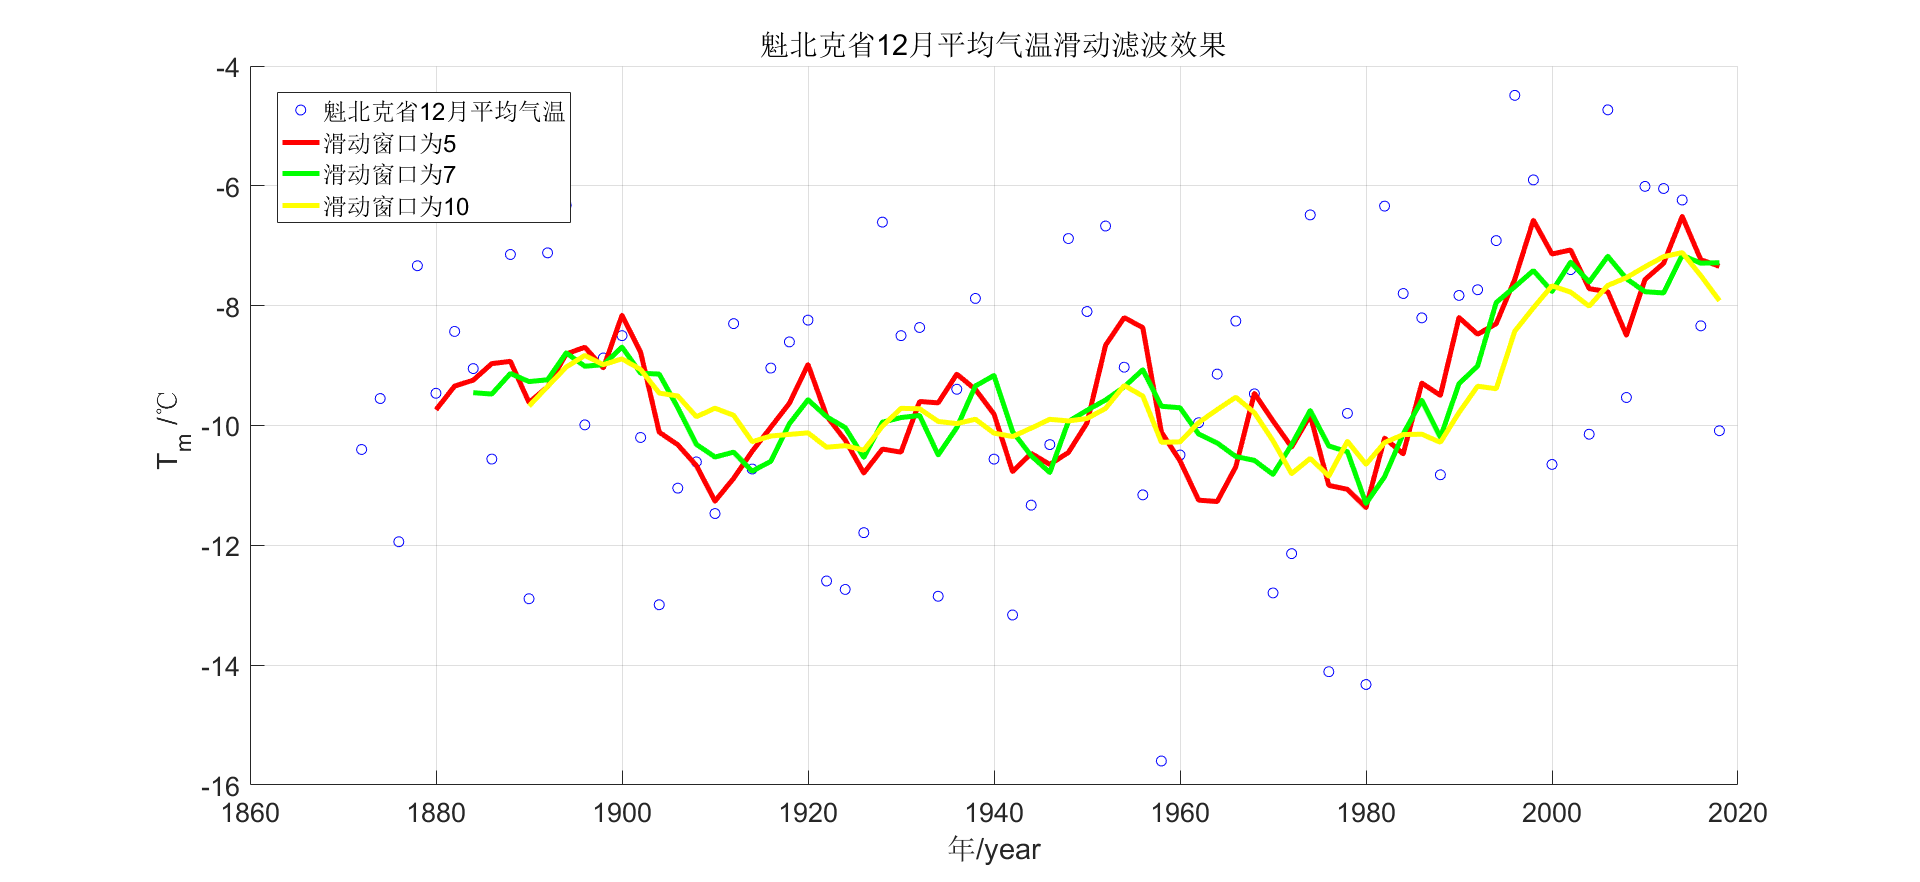
\includegraphics[width=\textwidth]{滑动滤波.png}
\caption{魁北克省12月平均气温滑动平均滤波}\label{slidewindow}
\end{figure}

由上图可知,滑动窗口越大,滑动滤波保留的原始数据的时间信息越模糊,因此我们采用五点滑动平均的方法估计数据变量的局部均值,使得变量的更新与一段时间内的历史取值相关联,并剔除年分辨率数据下的年际变值扰动。

该方法很好地保存了时间序列的长度,但是对于过强的年内信号无法彻底剔除。因此,我们使用傅里叶函数为基函数对时间序列进行逼近,将时域信号转换为频域信号,通过低通滤波来滤除相关噪声,获取期望的频域信号。之后,我们采取谐波滤波的方法,获得基准频率$\omega = 0.06998$,通过傅里叶反变换,将离散信号拟合为连续曲线,如图\ref{filter}所示。

\begin{figure}[ht]
\centering
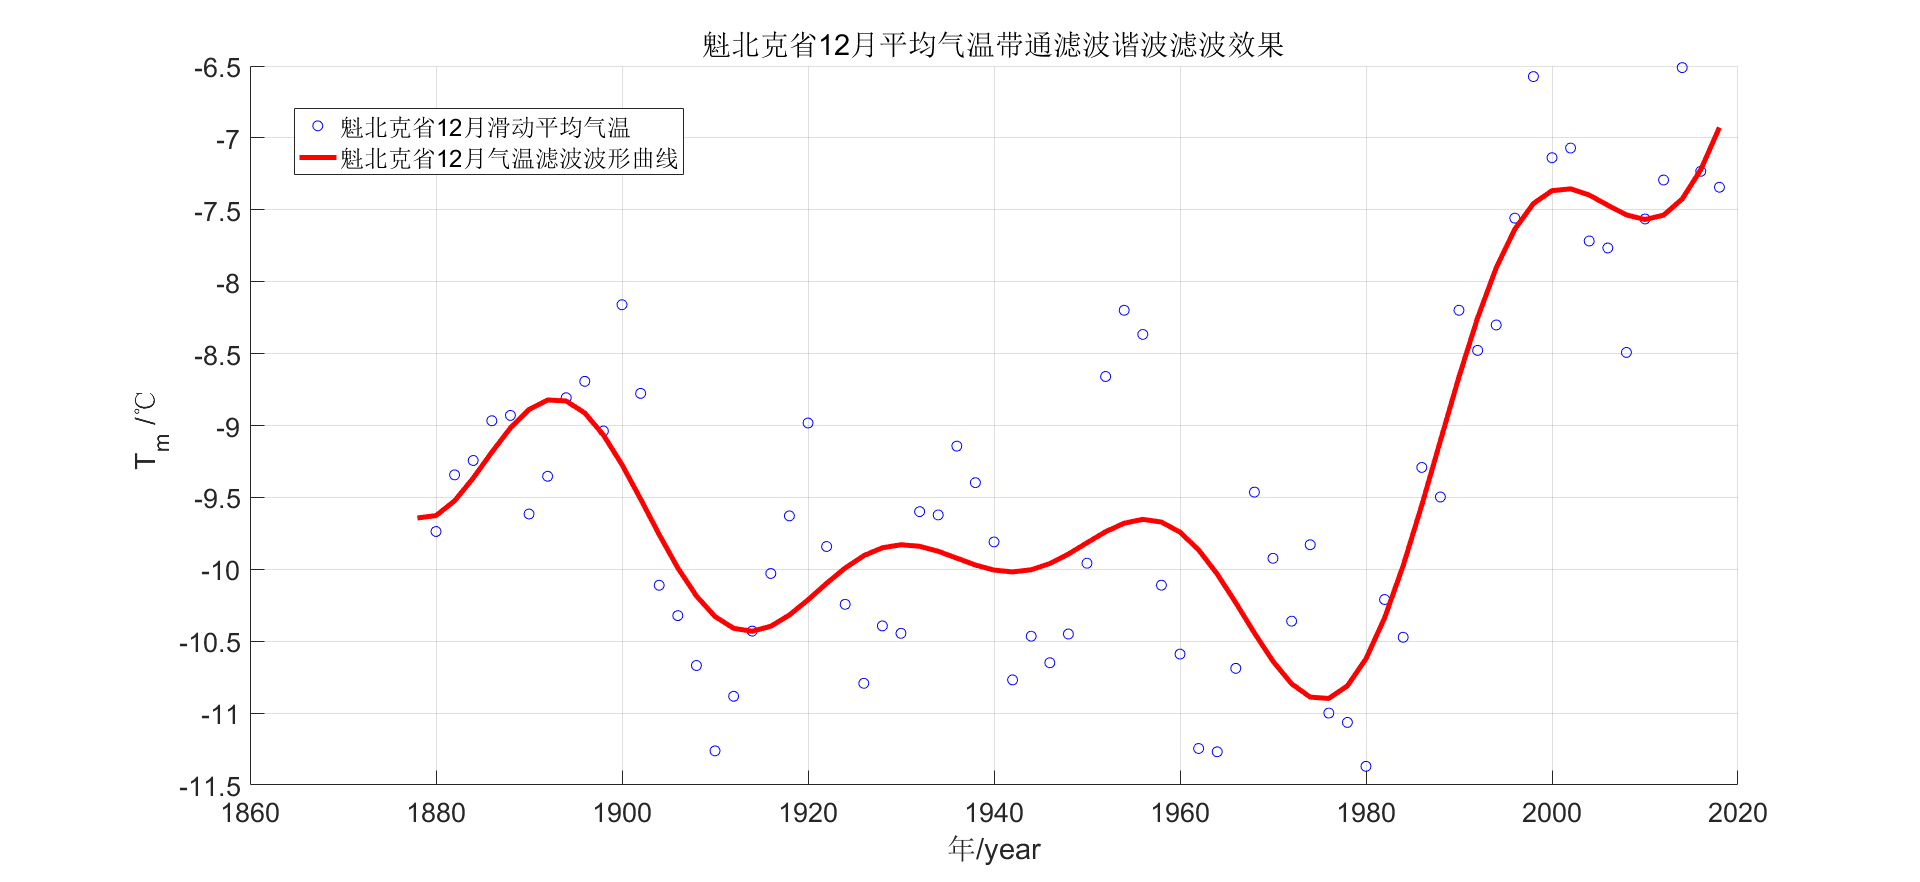
\includegraphics[width=\textwidth]{带通滤波.png}
\caption{魁北克省12月平均气温滤波效果}\label{filter}
\end{figure}

上图中滤波拟合曲线R-square=0.7433,RMSE=0.691,滤波拟合效果较好。图中可以看出,魁北克省12月平均气温存在一个20年左右的冷热周期。

我们在加拿大十三个省份中选取观测站数据最为完善的安大略省(Ontario)为例。我们拟合了安大略省从1870年到2018年,在3月、6月、9月、12月的$T_m$、$T_x$和$T_n$的变化趋势。由图\ref{ON}可知,在1890年以前,安大略省的四个季度的气温均有下降趋势,并在十九世纪末出现局部最低值。之后的二十世纪到二十一世纪初,安大略省四个季度的温度均有上升趋势,其中3月和12月,即春冬季节的温度上升趋势更加明显。此外,安大略省3月历史气温中,分别于1890、1920、1940、1980年左右遭遇春季寒潮。

\begin{figure}[ht]
\centering
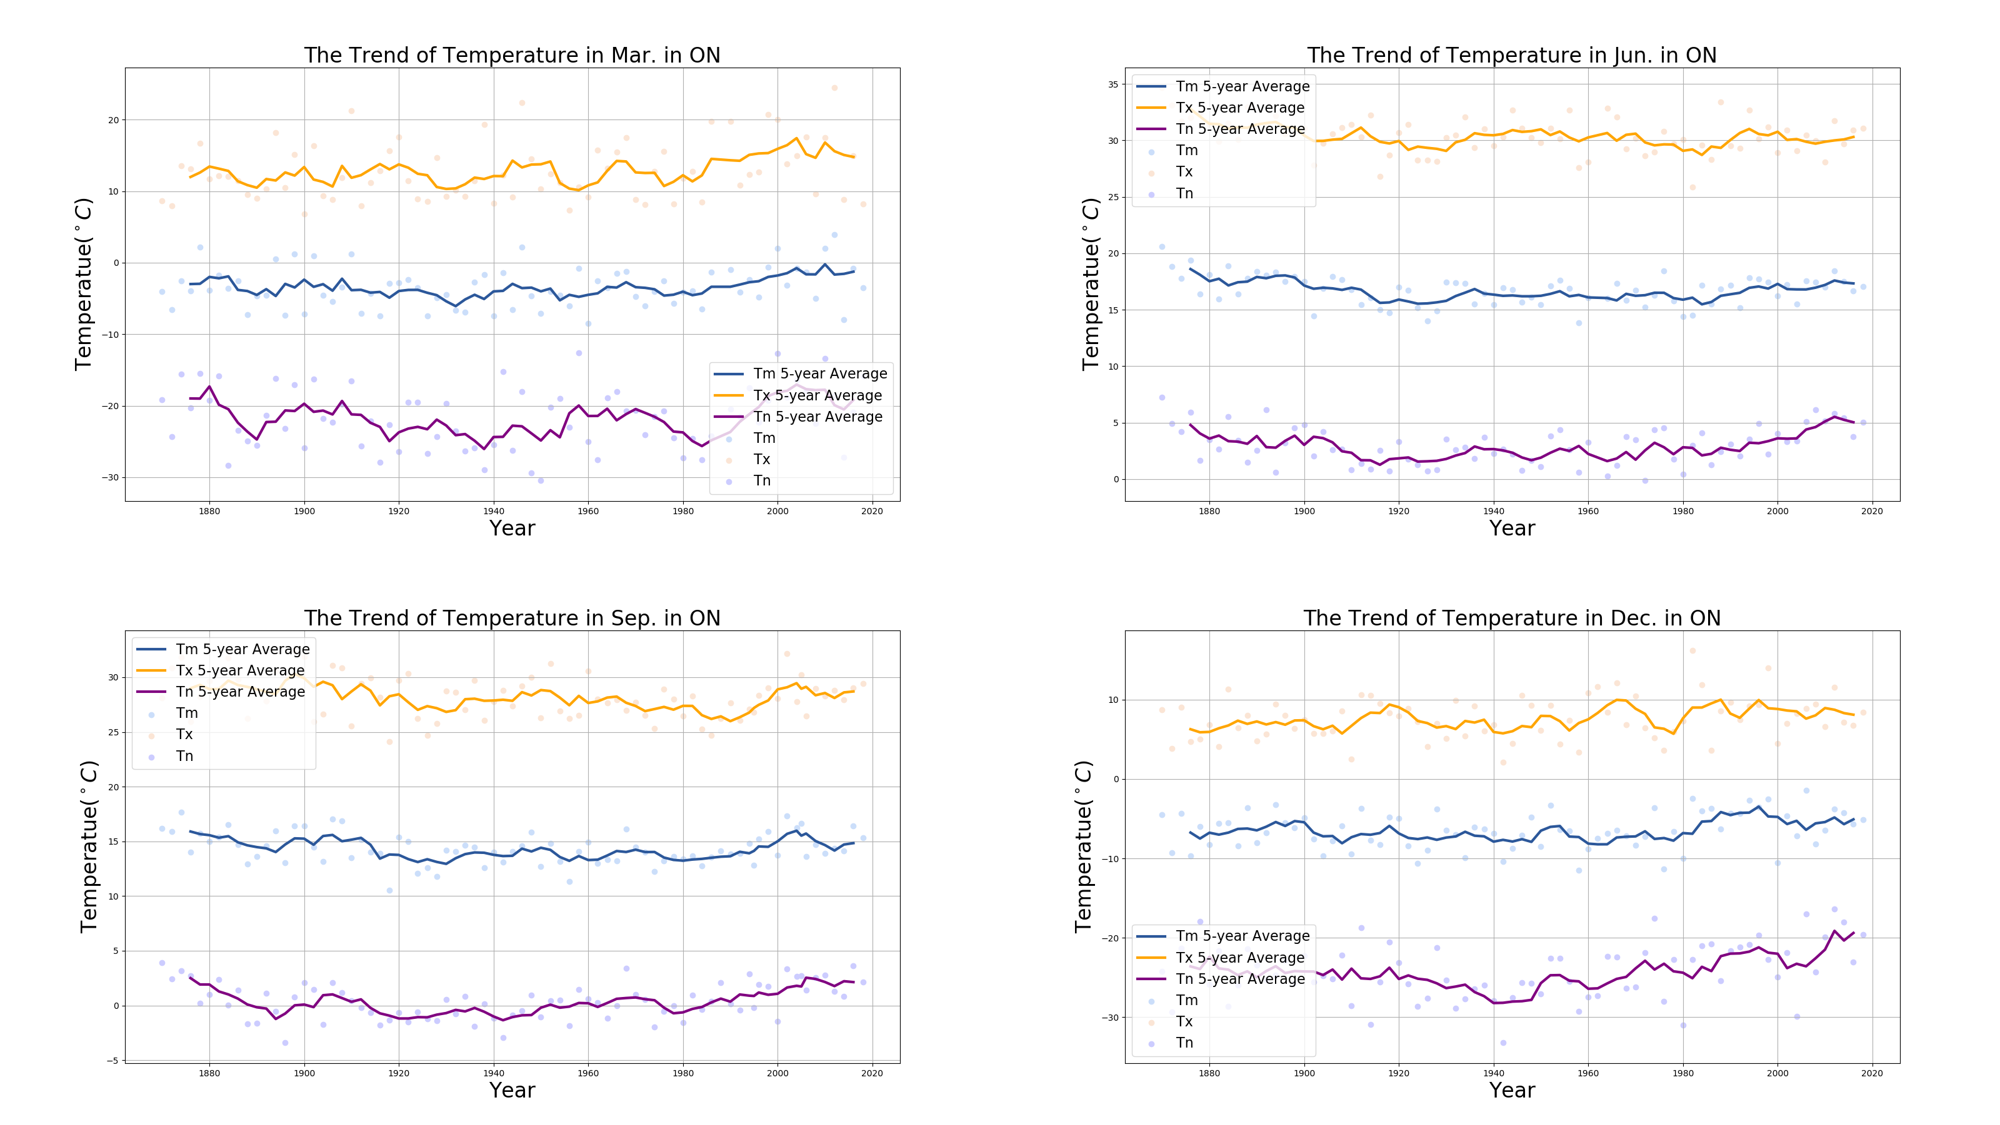
\includegraphics[width=\textwidth]{安大略省温度.png}
\caption{1870-2018年:安大略省在3月、6月、9月、12月的温度的变化趋势}\label{ON}
\end{figure}

为了挖掘加拿大温度的时空变化趋势,我们在加拿大四个地区各选择了一个省份作为代表,分别为纽纳瓦特省(北部)、爱德华王子岛省(东部海岸)、安大略省(五大湖地区)、育空地区(西部)。如图\ref{NU}所示,观察各个省份从1870至2018年的$T_m$、$T_x$和$T_n$的变化,发现各地区的温度均处于上升状态。其中,北方省份即纽纳瓦特省温度上升趋势最为明显,处于东南部宜居地区的爱德华王子岛省与安大略省冬季温波动较大。

\begin{figure}[ht]
\centering
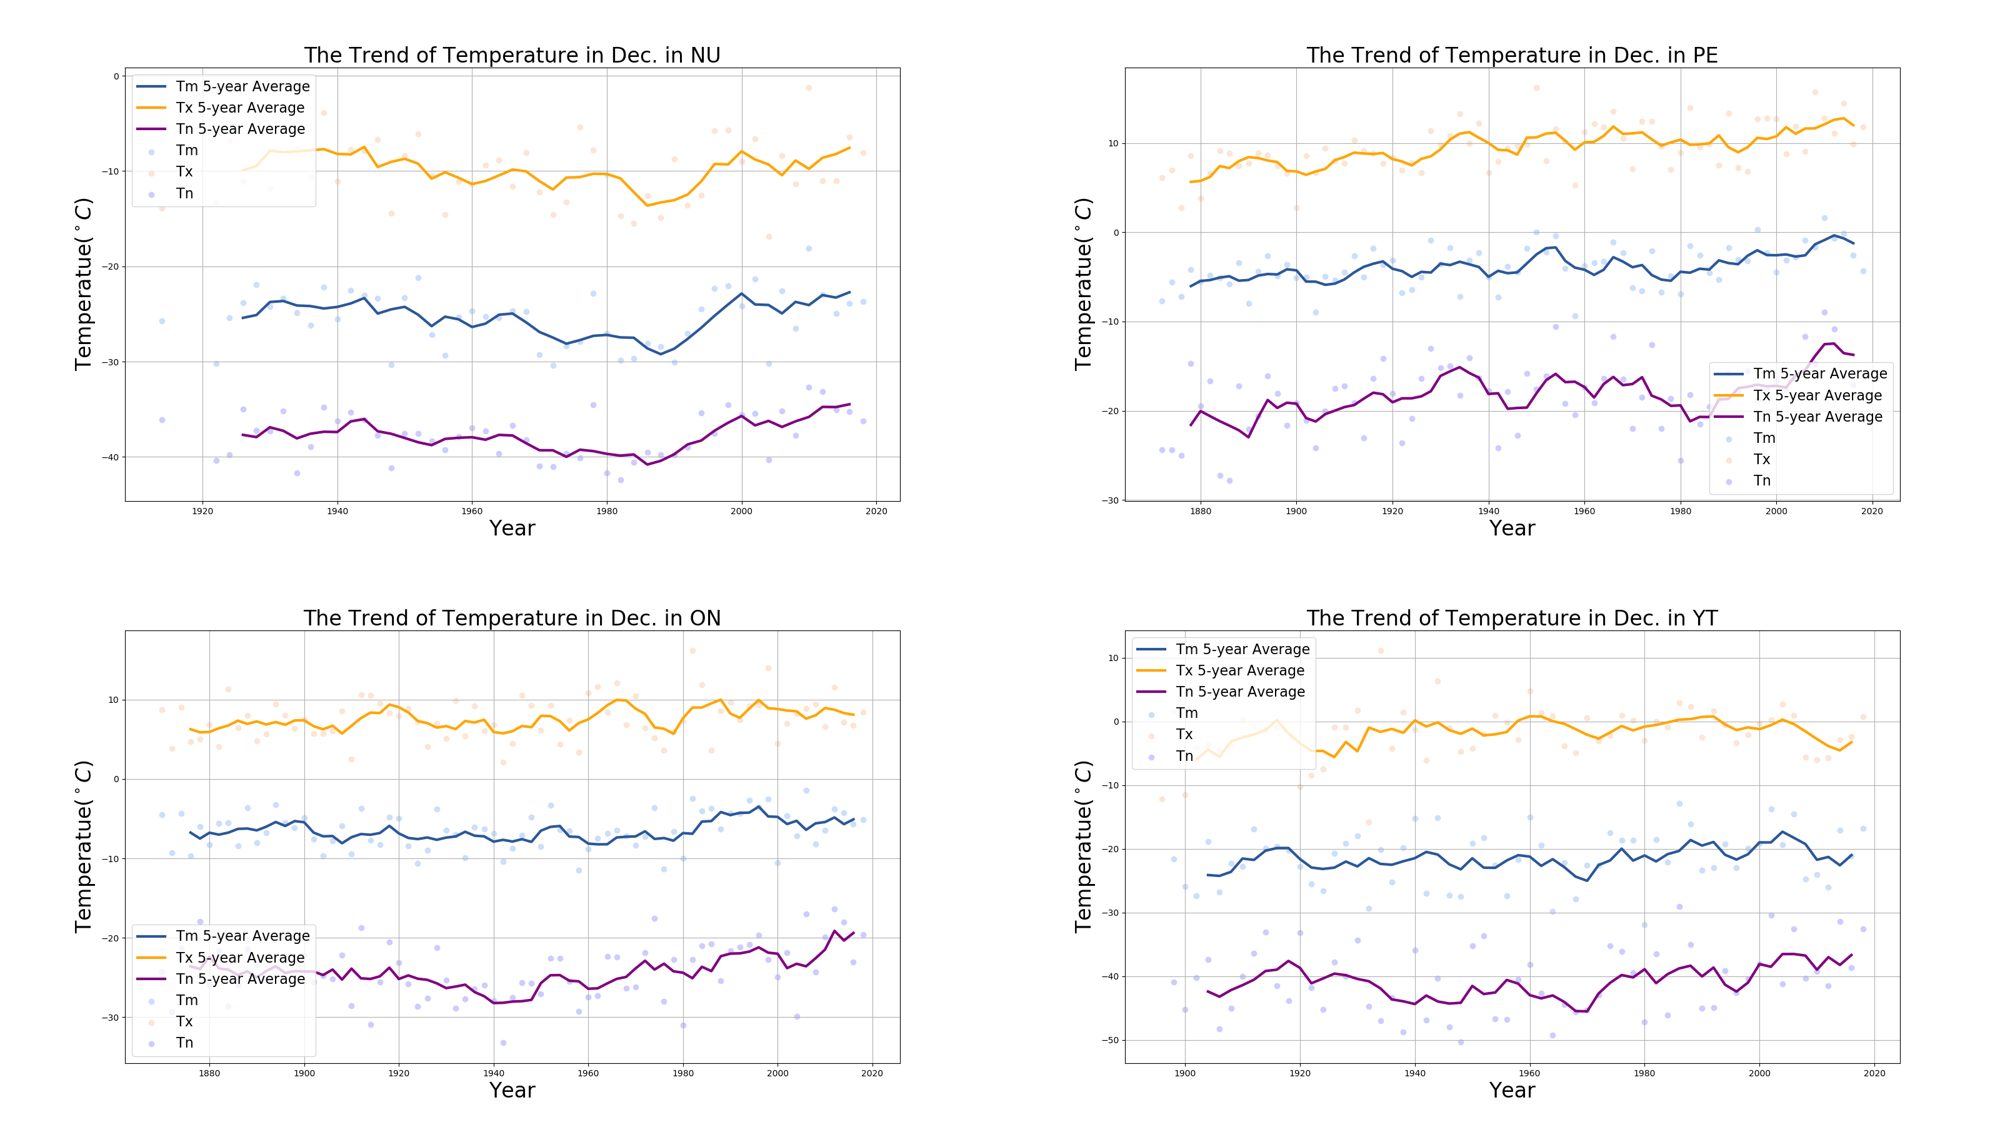
\includegraphics[width=\textwidth]{温度变化趋势.png}
\caption{1870-2018年:NU、PE、ON和YT在3月、6月、9月、12月的温度变化趋势}\label{NU}
\end{figure}

为了观测加拿大各省的气温变化趋势的空间关系,我们基于1870-2018年的$T_m$、$T_x$和$T_n$的数据,绘制了如图\ref{ave}和\ref{std}的平均气温分布图和平均气温标准差分布图。

\begin{figure}[p]
\centering
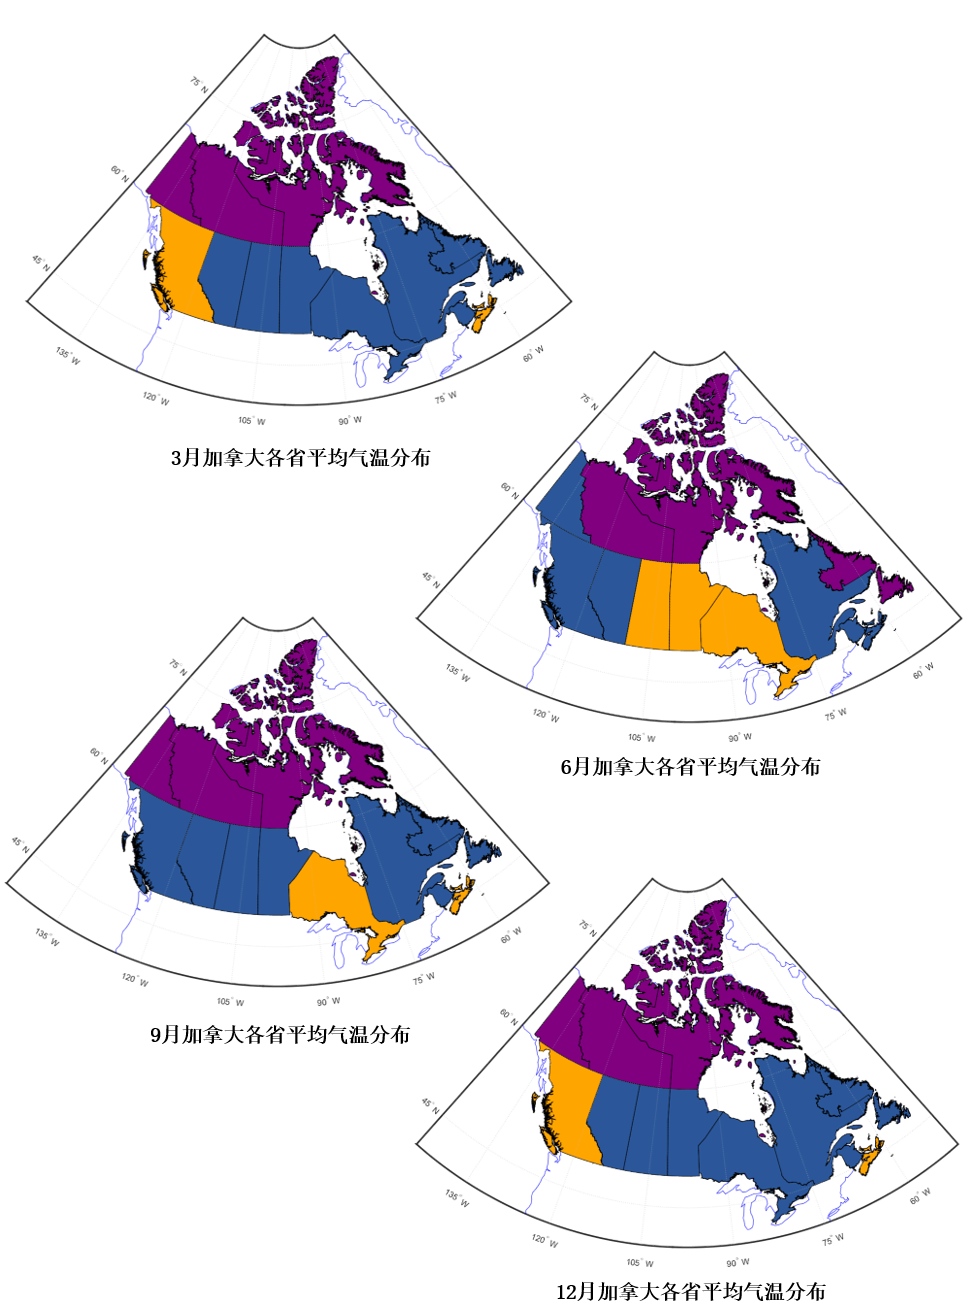
\includegraphics[width=\textwidth]{平均气温分布图.png}
\caption{加拿大各省在3月、6月、9月和12月的平均气温分布图}\label{ave}
\end{figure}

\begin{figure}[p]
\centering
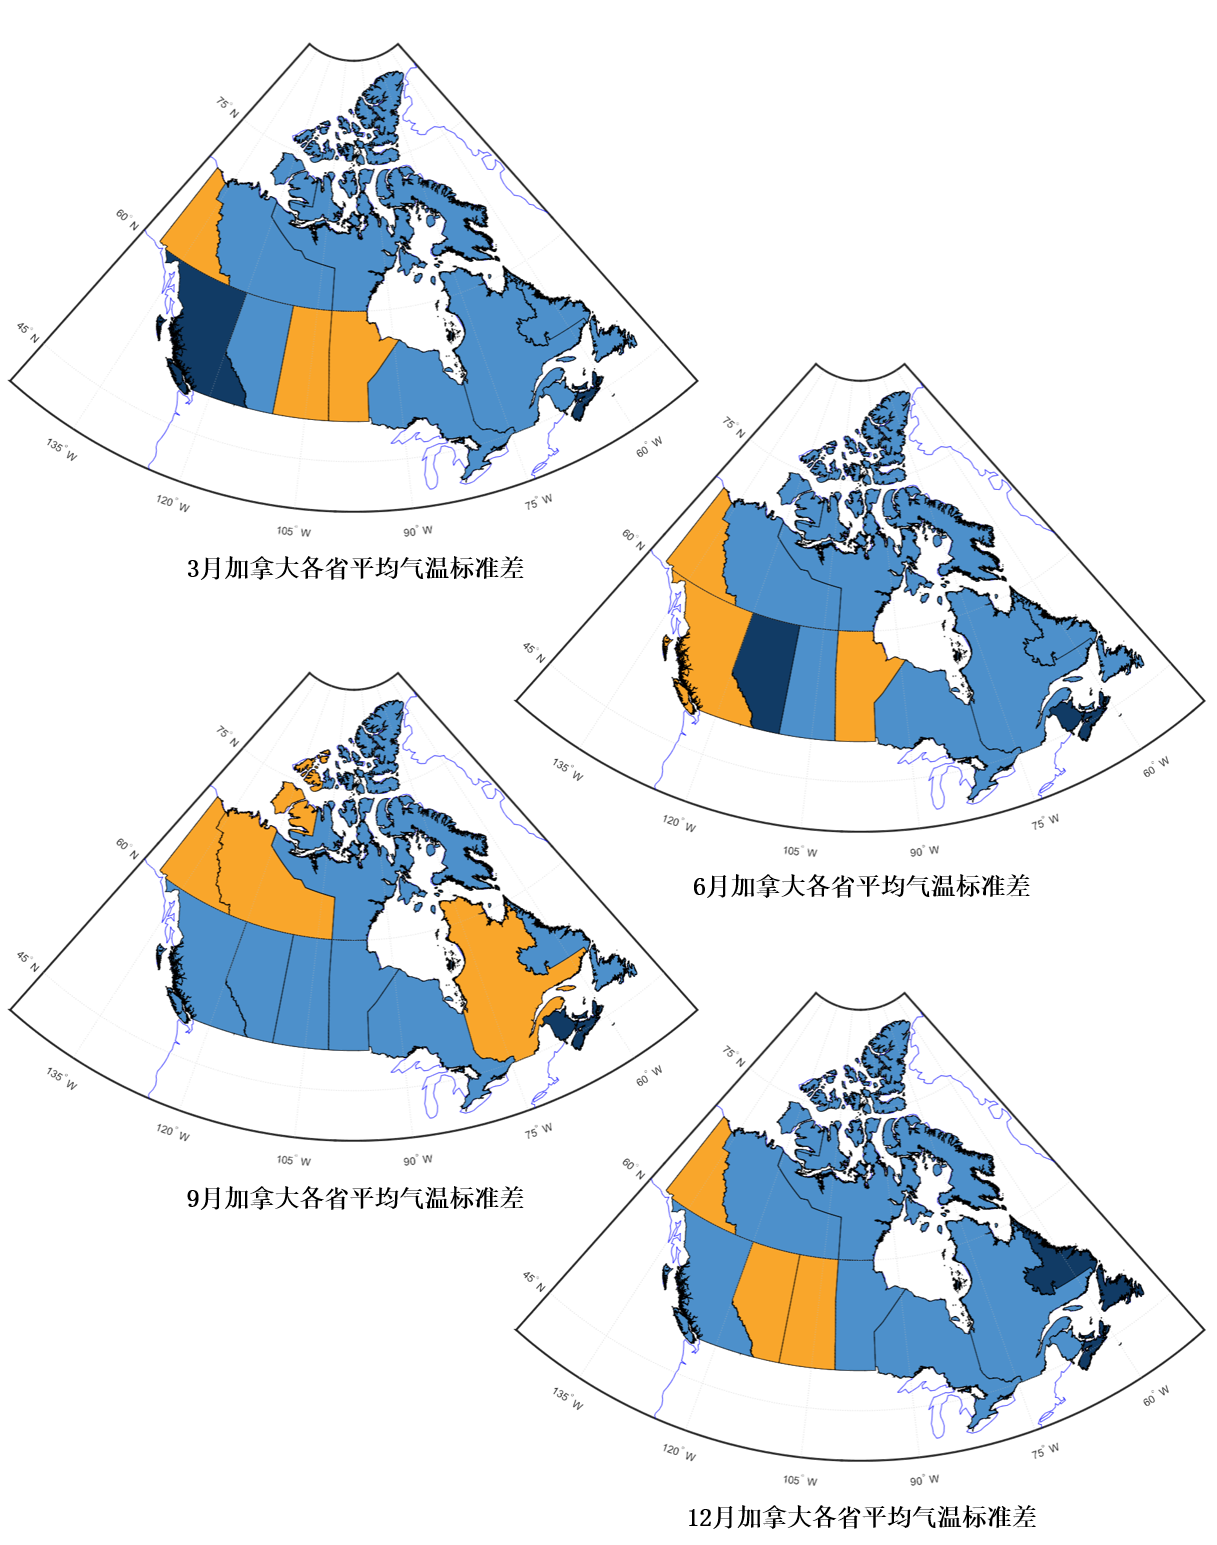
\includegraphics[width=\textwidth]{平均气温标准差分布图.png}
\caption{加拿大各省在3月、6月、9月和12月的平均气温标准差分布图}\label{std}
\end{figure}

在图\ref{ave}加拿大各省平均温度分布图中,我们选用暖黄色代表温度较高的区域,冷色调表温度较低的区域。观察可知,受北大平洋暖流、阿拉斯加暖流、北大西洋暖流影响,位于加拿大东西部海岸的不列颠哥伦比亚省和爱德华王子岛省冬季气温较为温和。

在图\ref{std}加拿大各省平均气温标准差分布图中,暖黄色代表这一部分区域历年的温度变化幅度较大,冷色调这一部分区域历年的温度标准差较小,无太大波动。

\subsubsection{海洋表面温度(SST)的变化规律}

海洋表面温度(Sea Surface Temperature,SST)是地球表面热特征之一,其会受到海洋内部和外部环境影响而产生变化,而SST发生变化后又会进一步对大气产生影响。因此分析其变化规律具有重要意义。所以针对任务二,我们对ESRL(地球系统研究实验室)所提供的SST数据进行统计分析,得出1850年至2015年海洋表面温度的变化规律。

通过计算海洋表面温度平均值,我们得到1850年到2015年每月全球平均SST随时间变化的趋势图\ref{sst_ave}。从图\ref{sst_ave}中可以看出,随着年份的增加,在达到600个月,即1900年,海洋表面温度达到最低值,而在1938 年,温度达到了一个极大值,且SST在这一阶段达到一个小峰值。但是在此之后全球平均SST便不断上升。并且通过滑动平均得到的每年海洋表面滑动平均温度的斜率也在不断变大,表明从第1100 个月,即1940年开始,海洋表面温度的上升速度也越来越快。

\begin{figure}[ht]
\centering
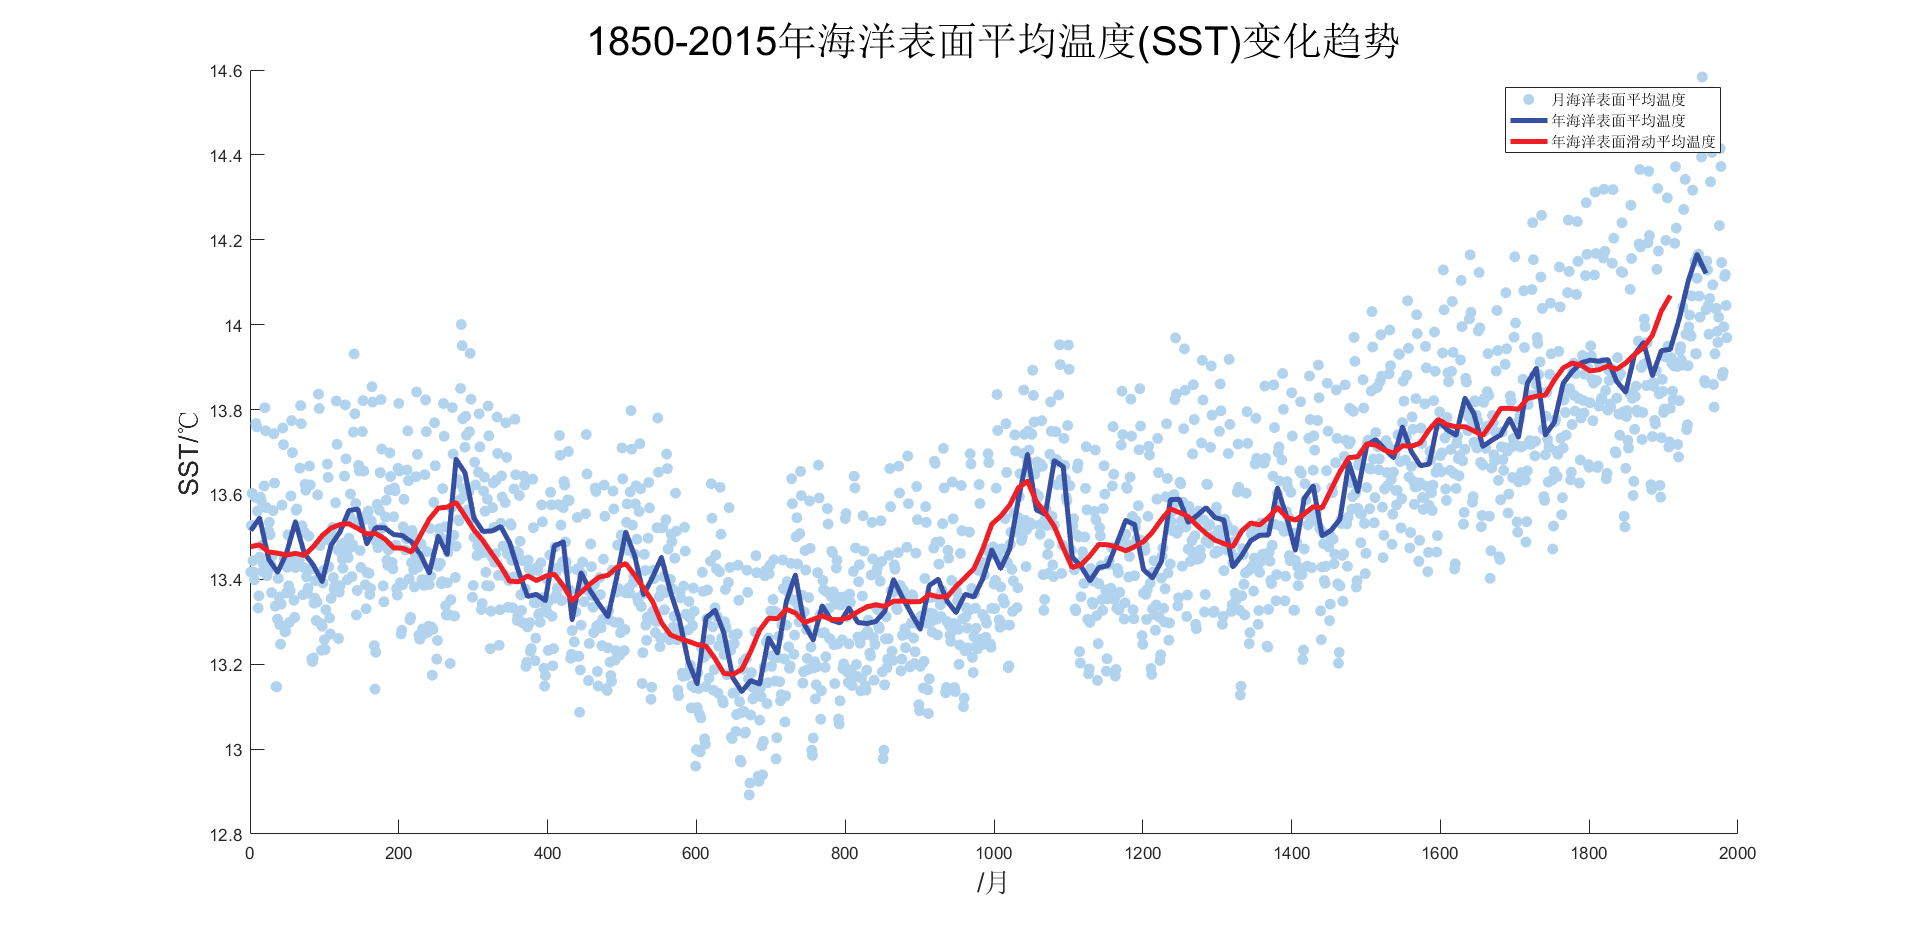
\includegraphics[width=\textwidth]{SST平均.png}
\caption{1850-2015年海洋表面平均温度的变化趋势}\label{sst_ave}
\end{figure}

通过计算海洋表面温度方差,我们得到1850年到2015年海洋表面温度方差分布图\ref{sst_std}。观察图\ref{sst_std}可知,全球海洋表面温度在北太平洋、北大西洋与赤道东部太平洋地区方差较大。北太平洋与北大西洋受中纬西风影响,形成北太平洋暖流与北大西洋暖流。赤道东部太平洋受赤道南北两侧东北信风与东南信风影响,形成北赤道暖流与南赤道暖流。上述洋流对海洋表面温度影响较大。

\begin{figure}[ht]
\centering
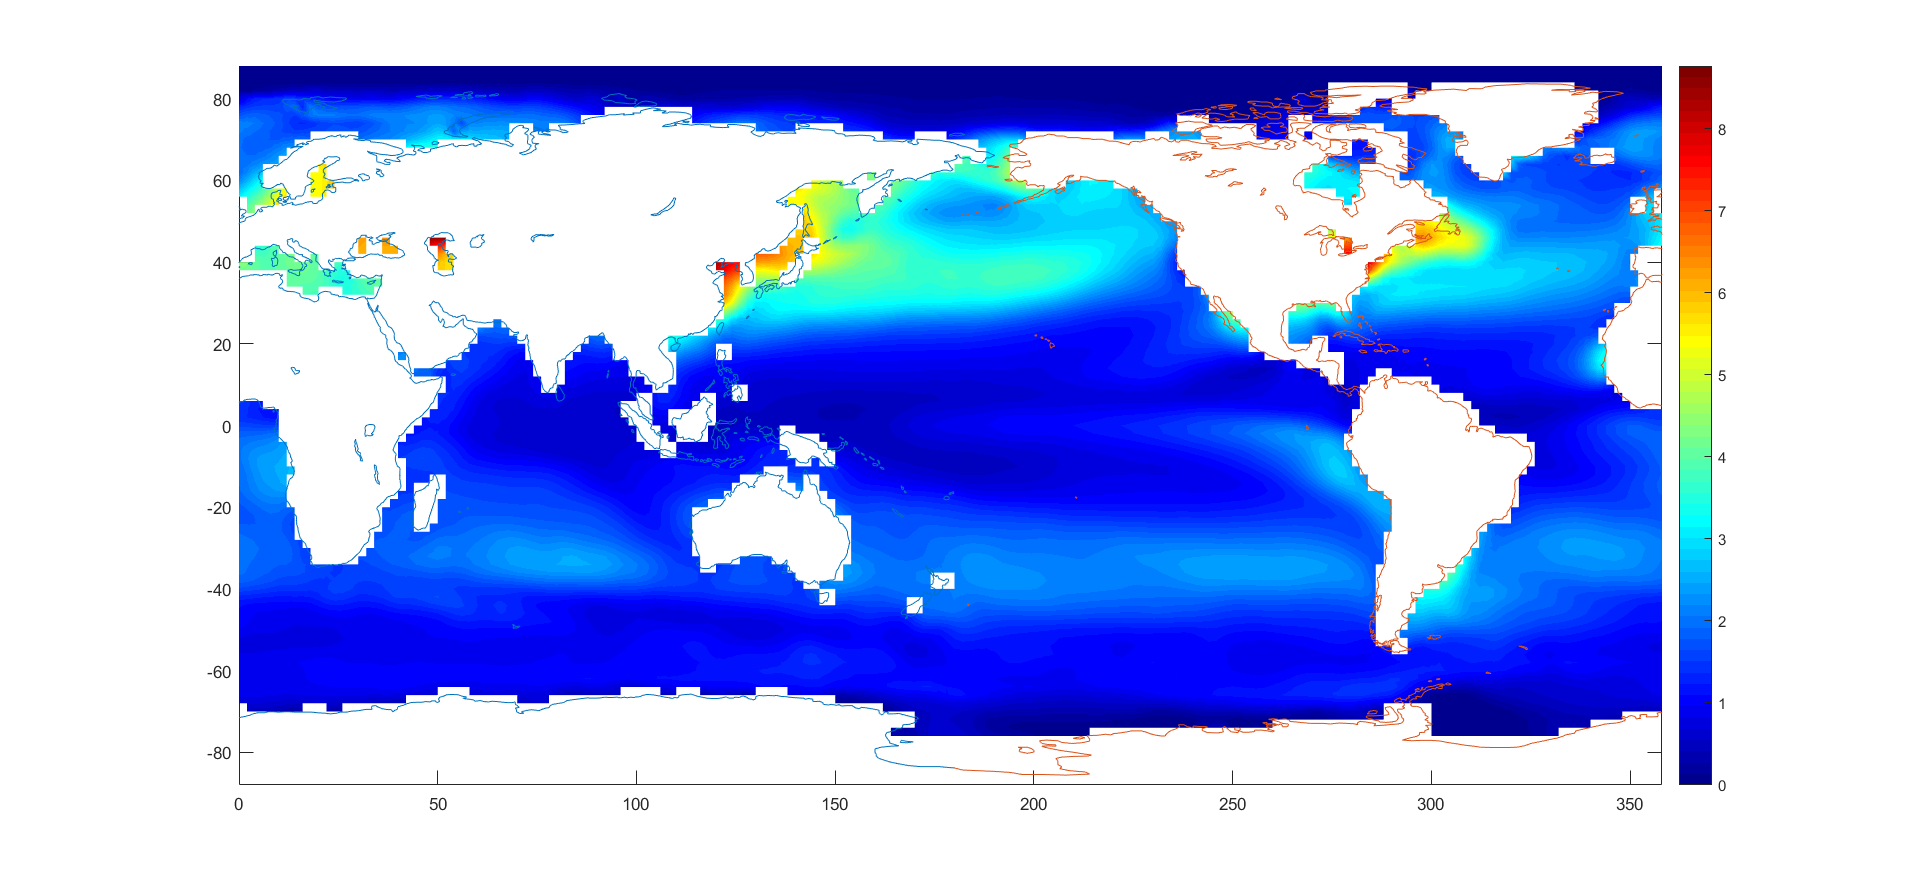
\includegraphics[width=\textwidth]{SST标准差Jet.png}
\caption{1850-2015年海洋表面平均温度方差分布}\label{sst_std}
\end{figure}

\section{问题二分析与建模}

\subsection{问题分析}

针对问题二,我们需要建立一个数学模型,借助模型来预测未来25年的气候变化,其中的影响因子包括地球的吸热、地球的散热以及海洋的温度。同时,我们需要找出相应的衡量标准,即哪些实际气象参数量需要被纳入到模型计算中,来表征题目中所要求的气象参数量。对于模型的确立,因为相关参数也随时间而变化,因此这里我们使用了偏微分方程的求解模型来初步推导未来25年下气象的变化。同时,因为该预测数据为气象数据\cite{Dunstone2010Impact},我们考虑使用EOF与PCA方法来进一步的推导与求解。来更完整的预测相应的变化趋势。

\subsection{问题求解}

我们先确定了每一个抽象物理量所针对的实际计量参数。首先,气候是长时间内气象要素和天气现象的平均或统计状态,时间尺度为月、季、年、数年到数十年,因此需要有足够的年份数据来支撑训练我们所设计的模型。我们将模型简化,将年平均气温作为气候的衡量指标,通过对未来25年全世界年平均气温的预测,来表征对未来25年气候变化的预测。其次,我们通过地气系统表层吸收的太阳辐射来间接表征地球的吸热;RCP浓度(浓度路径)来间接表征地球的散热;海洋表面温度来表征海洋的温度。

我们将问题二的模型抽象为一个“地气系统”预测分析模型,在该地气系统中包含太阳辐射总输入、大气反射、大气向太空辐射值,地面向大气辐射值、大气向地面辐射值,如图\ref{ea_sys}所示。而通过分析,得到RCP 浓度(浓度路径)会影响大气向地面的辐射值,以及地面向大气的辐射值。而地面向大气的辐射、大气向地面的辐射和所吸收的太阳辐射值都会影响到地球表面温度,而海洋表面温度则会更为直接的影响地球表面温度\cite{Mochizuki2010Pacific}。

\begin{figure}[ht]
\centering
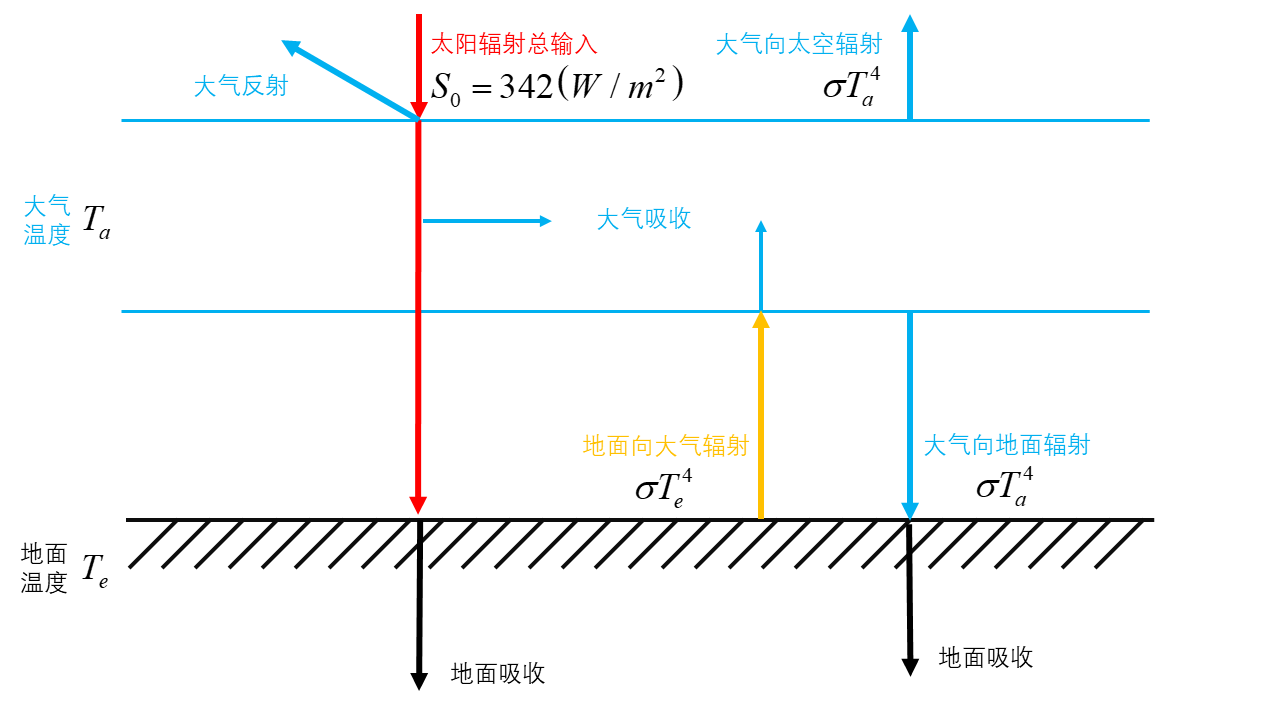
\includegraphics[width=\textwidth]{地气系统.png}
\caption{地气系统热量图}\label{ea_sys}
\end{figure}

\subsubsection{系统模型的建立}

地球表面温度可以由偏微分方程表达。

\begin{equation}
\left\{
\begin{array}{c}
\frac{\partial {T_e}}{\partial {x}} = g(T_e, T_a, x) \\
\frac{\partial {T_a}}{\partial {x}} = f(T_e, T_a, x) \\
\end{array}
\right. 
\end{equation}

其中$T_e$为地球表面温度,$T_a$为大气温度,$x$为影响因素。对于$x$,我们主要考查海洋表面温度模态与主要温室气体代表路径浓度的特征。

\subsubsection{海洋表面温度(SST)模态分析}

正交函数分析方法(Empirical Orthogonal Function,EOF)也称特征向量分析(eigenvector analysis),是一种分析矩阵数据中的结构特征,提取主要数据特征量的一种方法。而特征向量对应的是空间样本,也称空间特征向量或者空间模态(EOF),在一定程度上反映要素场的空间分布特点;主成分对应的是时间变化,反映相应空间模态随时间的权重变化。EOF有时也称作时空分解,即$X = EOF_{m \times n} \times PC_{m \times n}$其中$m$是空间点,$n$是时间序列长度。

我们利用EOF方法对1850-2005年共计16020个观测点、1985月海洋表面温度$SST_{m \times n}$进行分析,其中$m=16020$,$n=1985$,算法如\ref{EOF}。

\begin{algorithm}[ht]
\caption{EOF方法}
\label{EOF}
\begin{algorithmic}[1]
\State Input: $X_{m \times n}$ 
\State 标准化 $X_{m \times n}$ 
\State $C_{m \times m} = \frac{1}{n} X_{m \times n} \times X_{m \times n}^T$
\State 计算方阵 $C_{m \times m}$的特征值$(\lambda_1, ..., \lambda_m)$与特征向量$V_{m \times m}$
\State 将特征值按从大到小的顺序排序$\lambda_1 > \lambda_2 > ... > \lambda_m$。
\State 得到非零特征根对应的特征向量$EOF$
\end{algorithmic}
\end{algorithm}

首先标准化$SST_{m \times n}$。计算相关系数矩阵

\begin{equation}
C_{m \times m} = \frac{1}{n} SST_{m \times n} \times SST_{m \times n}^T.
\end{equation}

计算相关系数矩阵特征值$(\lambda_1, ..., \lambda_m)$与特征向量$V_{m \times m}$,使

\begin{equation}
C_{m \times m} \times V_{m \times m} = V_{m \times m} \times E_{m \times m}.
\end{equation}

其中$E$是$m \times m$对角阵,即

\begin{equation}
E_{m \times m} = 
    \begin{bmatrix}
    \lambda_1 & 0 & \cdots & 0 \\
    0 & \lambda_2 & \cdots & 0 \\
    \cdots & \cdots & \cdots & \cdots\\
    0 & 0 & \cdots & \lambda_m \\
    \end{bmatrix}.
\end{equation}

各个特征值与特征向量贡献了如表\ref{SST_EOF}所示。

\begin{table}[ht]
\centering
\caption{全球SST EOF分解的前10个特征向量贡献率}\label{SST_EOF}%添加标题 设置标签
\begin{tabular}{cccccc}
\toprule  %添加表格头部粗线
模态& 特征值& 方差贡献率& 累计方差贡献率& 特征根误差下限& 特征根误差上限\\
\midrule  %添加表格中横线
1& 6651.313993& 0.613446& 0.613446& 6440.135& 6862.493\\
2& 705.3822621& 0.065057& 0.678503& 682.9864& 727.7782\\
3& 458.4528136& 0.042283& 0.720786& 443.8969& 473.0087\\
4& 298.0811611& 0.027492& 0.748278& 288.6171& 307.5452\\
5& 229.7952259& 0.021194& 0.769472& 222.4992& 237.0912\\
6& 180.0869910& 0.016609& 0.786081& 174.3692233& 185.8047587\\
7& 125.3396816& 0.011560& 0.797641& 121.3601427& 129.3192205\\
8& 98.0017317& 	0.009039& 0.806680& 94.89017365& 101.1132898\\
9& 89.6314432& 	0.008267& 0.814946& 86.78564199& 92.47724432\\
10& 79.3408031& 0.007318& 0.822264& 76.82173012& 81.85987615\\
\bottomrule %添加表格底部粗线
\end{tabular}
\end{table}

取前四个模态下的特征向量,并将其展开在二维的全球经纬度平面上如图\ref{v1m} \ref{v2m} \ref{v3m} \ref{v4m}所示。

其中,图\ref{v1m}表征的第一模态为南北半球气温周期性差异\cite{Mochizuki2010Pacific},相近颜色呈正相关,相反色系之间呈负相关。

\begin{figure}[!h]
\centering
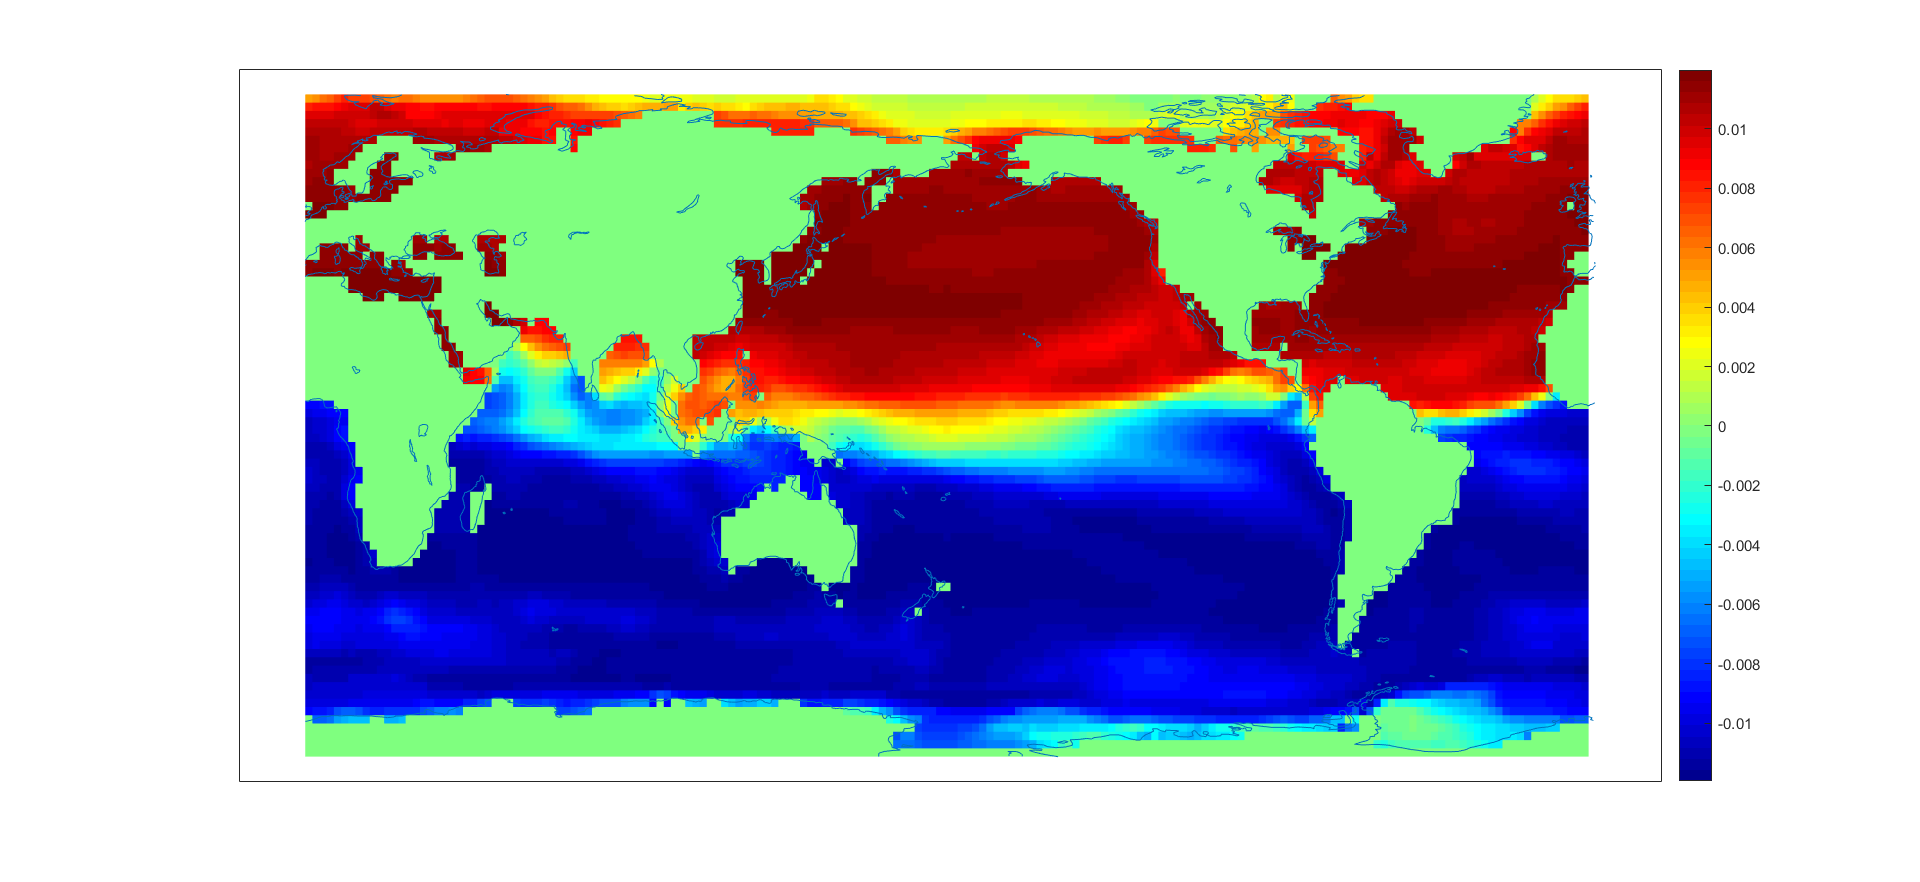
\includegraphics[width=\textwidth]{v1_model.png}
\caption{1850—2015年全球SSTA的EOF分解第一模态的空间分布}\label{v1m}
\end{figure}

SST的EOF第二模态的空间分布如图\ref{v2m}所示,表现为,在太平洋海区,赤道中东太平洋为正异常的高值中心,与南北太平洋中纬度海区呈负相关,这种空间分布与单独对太平洋SST做EOF分解得到的第一模态的空间分布型类似,该模态也是前人研究中指出的热带太平洋强迫中纬度太平洋的模态。该模态在热带印度洋呈现为“海盆一致模”,也就是印度洋海盆模态(Indian Ocean Basin Mode,IOBM),它是印度洋对太平洋 ENSO的响应模态。在南海及菲律宾以东海域 SSTA 也与赤道东太平洋同号;热带大西洋则表现为除了赤道东大西洋SST与赤道东太平洋反相外,其余海域则同相。

这是由于当厄尔尼诺现象出现后,加热的赤道东太平洋大气会出现Kelvin波的响应,这个异常信号会传到热带大西洋、印度洋,作用于当地的大气从而使得SST正异常;此外赤道东太平洋SST正异常会引起赤道大西洋东风加强,赤道东大西洋温跃层变浅\cite{Dunstone2010Impact},SST负异常;以及南海冬季风减弱SST正异常\cite{Nicholls1999Cognitive}。

\begin{figure}[ht]
\centering
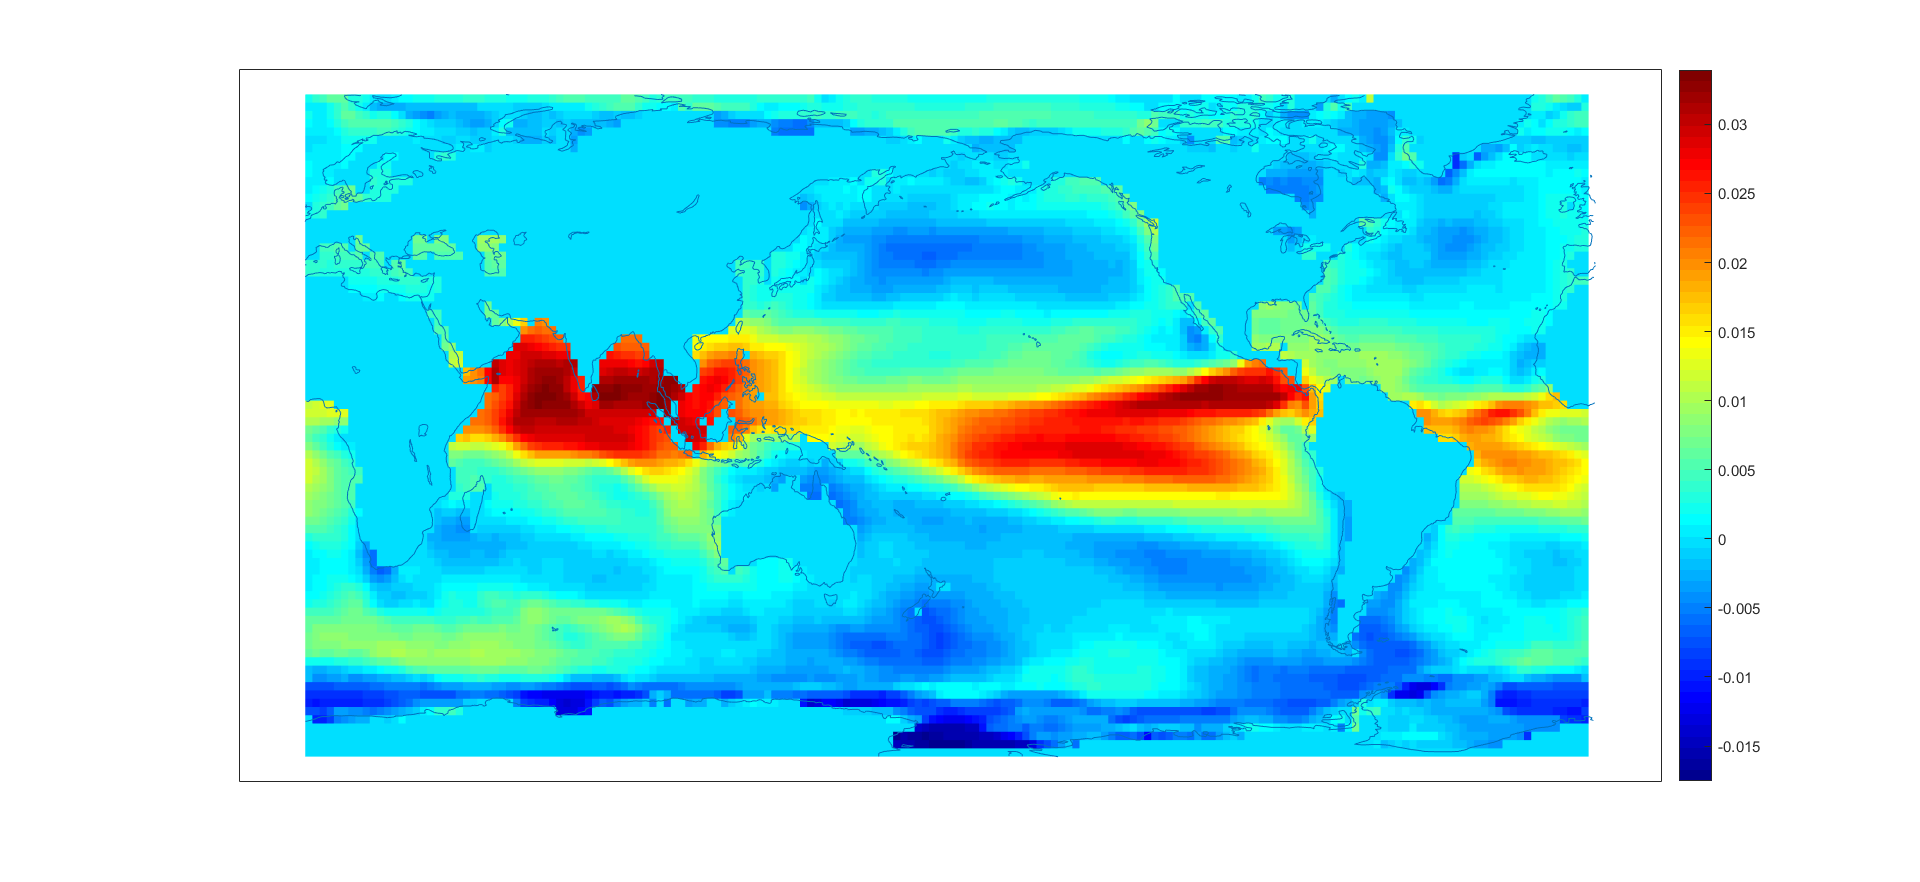
\includegraphics[width=\textwidth]{v2_model.png}
\caption{1850—2015年全球SSTA的EOF分解第二模态的空间分布}\label{v2m}
\end{figure}

全球SST的EOF第三模态空间分布如图\ref{v3m}所示,当赤道中东太平洋与北太平洋SST为正异常的高值中心时,赤道东大西洋与北大西洋负异常,在全球尺度上形成了太平洋-大西洋联合的双偶极子结构。大西洋SSTA的空间分布与泛大西洋年代际振荡的大西洋从北到热带大西洋的三极分布较一致。北太平洋和热带太平洋都有东西异常反号的特征,大西洋偏向于同相,印度洋的SST虽然有东西之间的差异,但整体同相。总体来说太平洋和大西洋反相\cite{Dunstone2010Impact},共同构成了太平洋-大西洋联合模态。

赤道中东太平洋和赤道大西洋SSTA的反相会产生跨越南美大陆的纬向风异常,通过大气桥建立了赤道中东太平洋和赤道大西洋SST之间的联系。目前中纬度太平洋-大西洋的偶极子尚未被讨论,后者可能代表了中纬度大气环流异常信号共同影响海洋的结果。

\begin{figure}[ht]
\centering
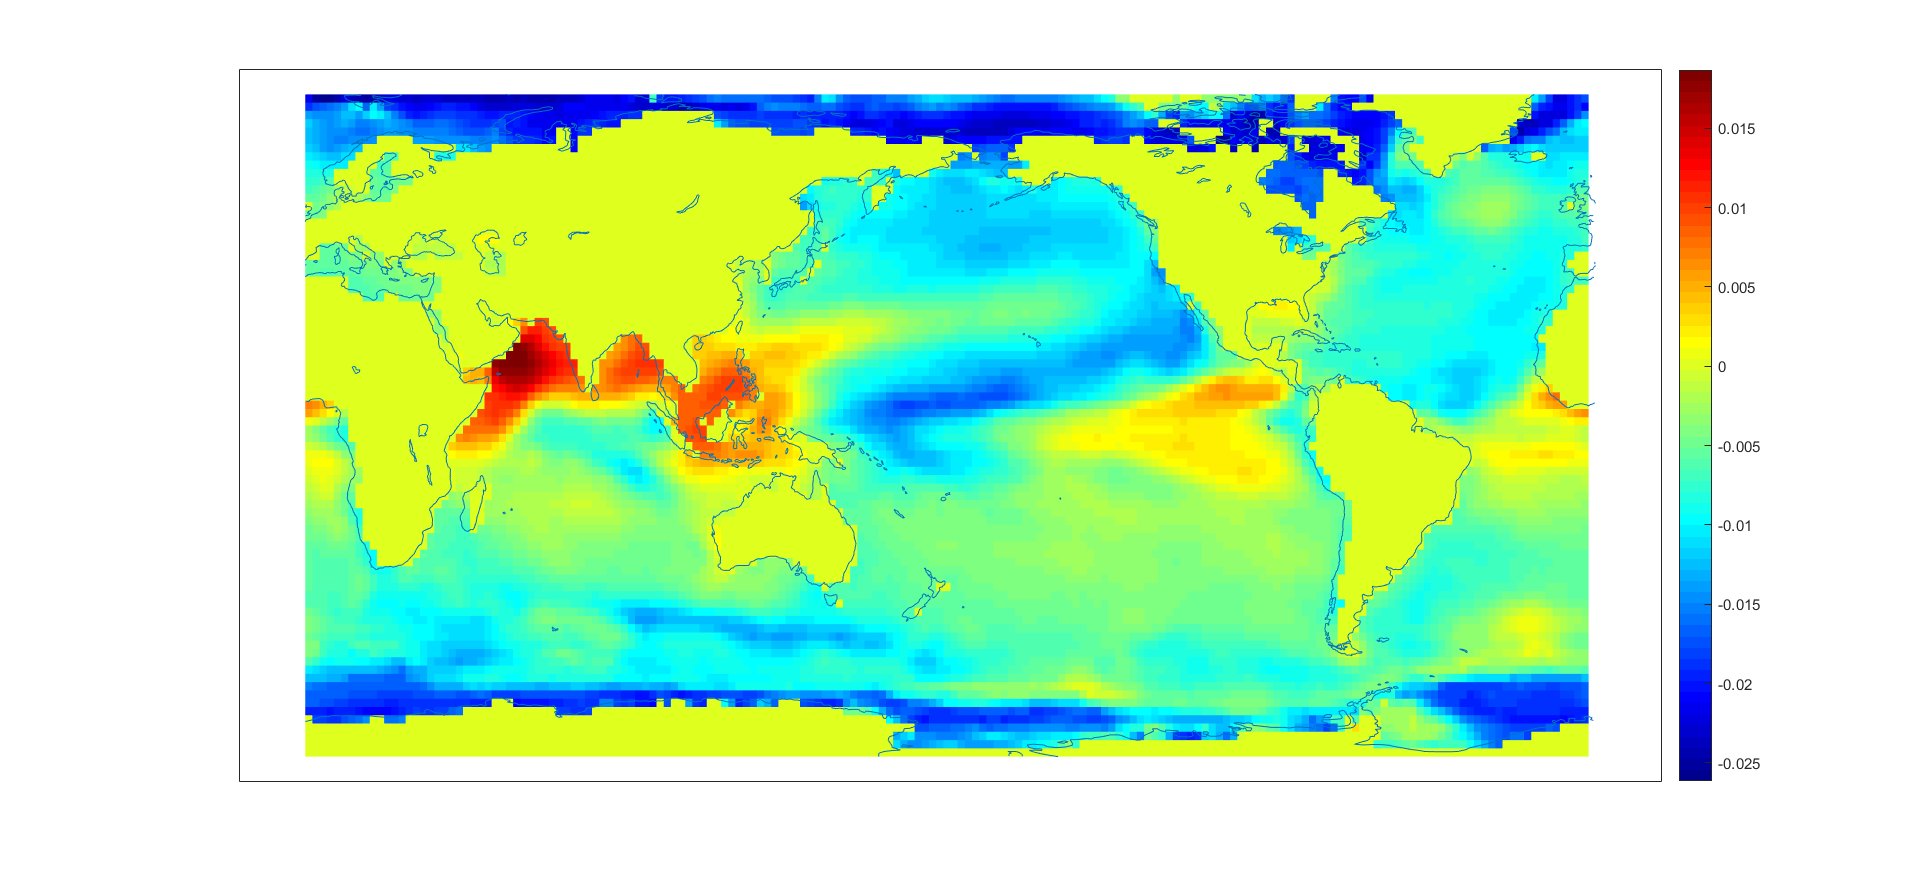
\includegraphics[width=\textwidth]{v3_model.png}
\caption{1850—2015年全球SSTA的EOF分解第三模态的空间分布}\label{v3m}
\end{figure}

该模态在100年内可以分为3个阶段,分别是1900—1927年、1928—1963年、1964—1995 年。可以看出,第1和第3个阶段北太平洋和赤道中东太平洋SSTA为正、北大西洋和热带大西洋为负;第2个阶段则相反,周期约为70年。对 SSTA的EOF分解的第二模态相应的时间系数进行小波分 析和功率谱分析后得到,该模态也有2~8a年际变化,该周期变化在80年代比较明显。

根据以上的分析和与第一主模态的比较表明,太平洋年代际变化影响大西洋,也有可能是大西洋全球SSTA第二主模态是以70年周期为主的模态,年代际变化影响太平洋。两者之间的关系尚未确在太平洋与大西洋上都有较明显的信号\cite{St2009Climate}。

\begin{figure}[ht]
\centering
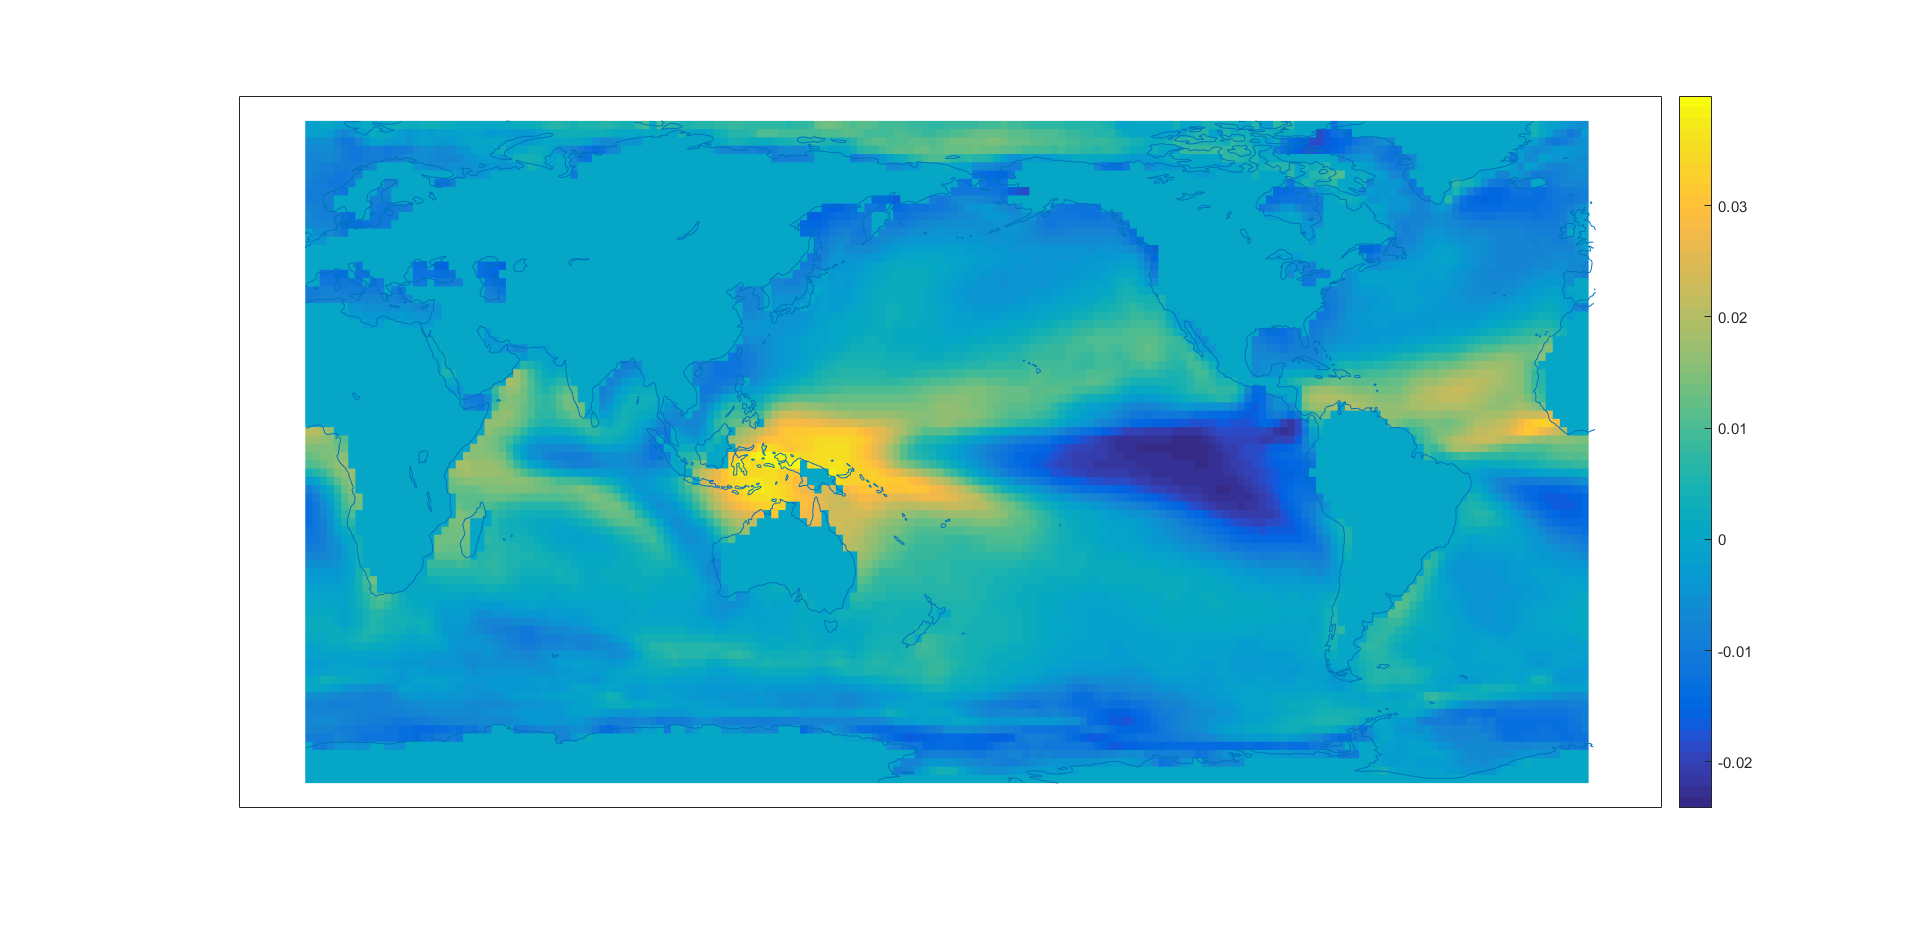
\includegraphics[width=\textwidth]{v4_model.png}
\caption{1850—2015年全球SSTA的EOF分解第四模态的空间分布}\label{v4m}
\end{figure}


经上述分析,我们取前模态对应的时间序列作为影响全球未来25年全球气候变化的主要因素\cite{Hastenrath1995Recent}。

\subsubsection{代表路径浓度(RCP)分析}

对于代表路径浓度RCP,我们选用其中11种主要温室气体大气浓度作为研究对象,其1765年至今增长趋势如图\ref{rcp_1765_2018}所示。

\begin{figure}[!h]
\centering
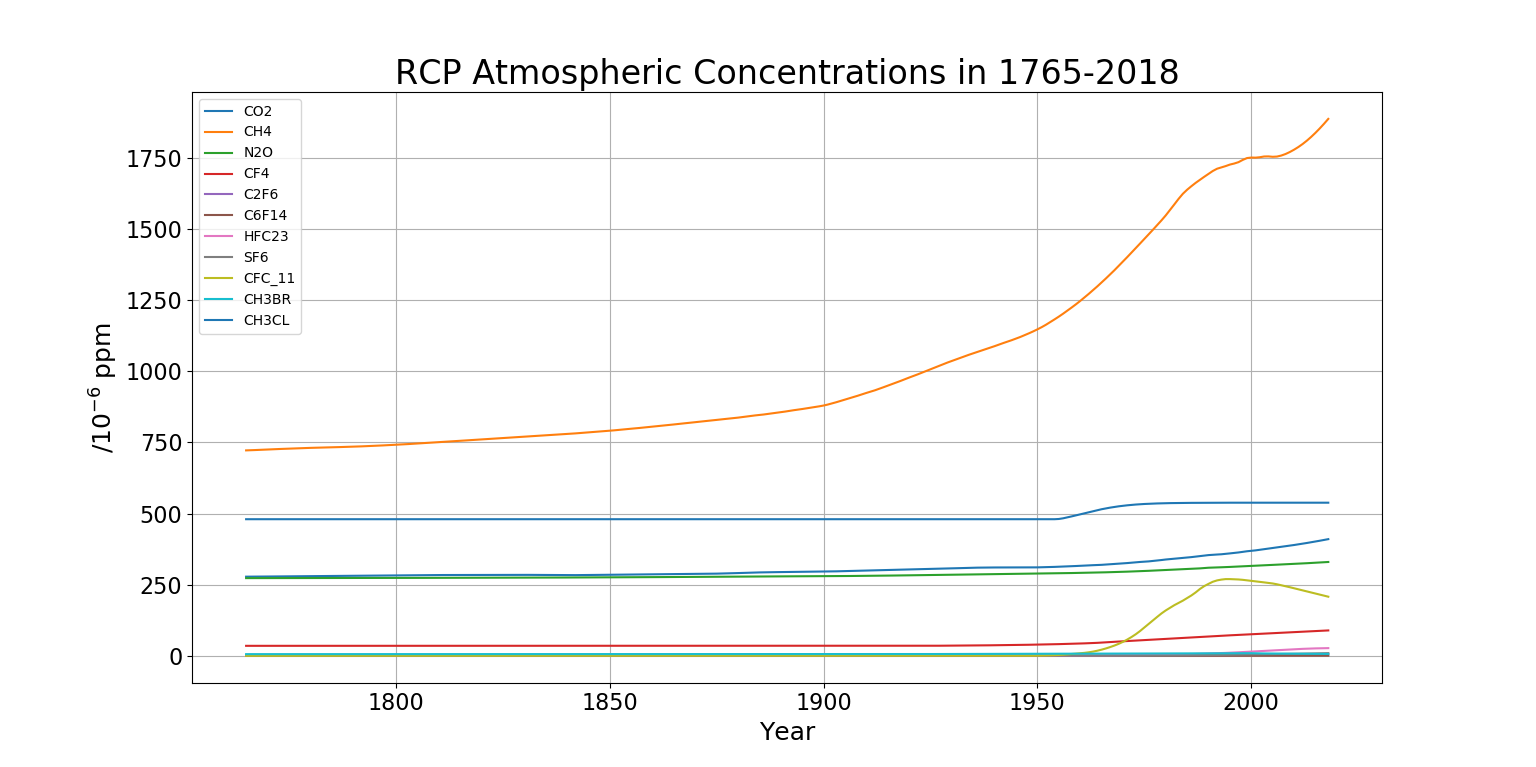
\includegraphics[width=\textwidth]{rcp_1765_2018.png}
\caption{1765-2018年RCP增长趋势}\label{rcp_1765_2018}
\end{figure}

目前已有多个模型预测RCP在未来的增长趋势,我们分别选用RCP6作为温室气体排放的乐观模型,如图\ref{rcp6}所示;RCP85作为温室气体排放的悲观模型,如图\ref{rcp85}所示\cite{Hastenrath1995Recent}。

\begin{figure}[!h]
\centering
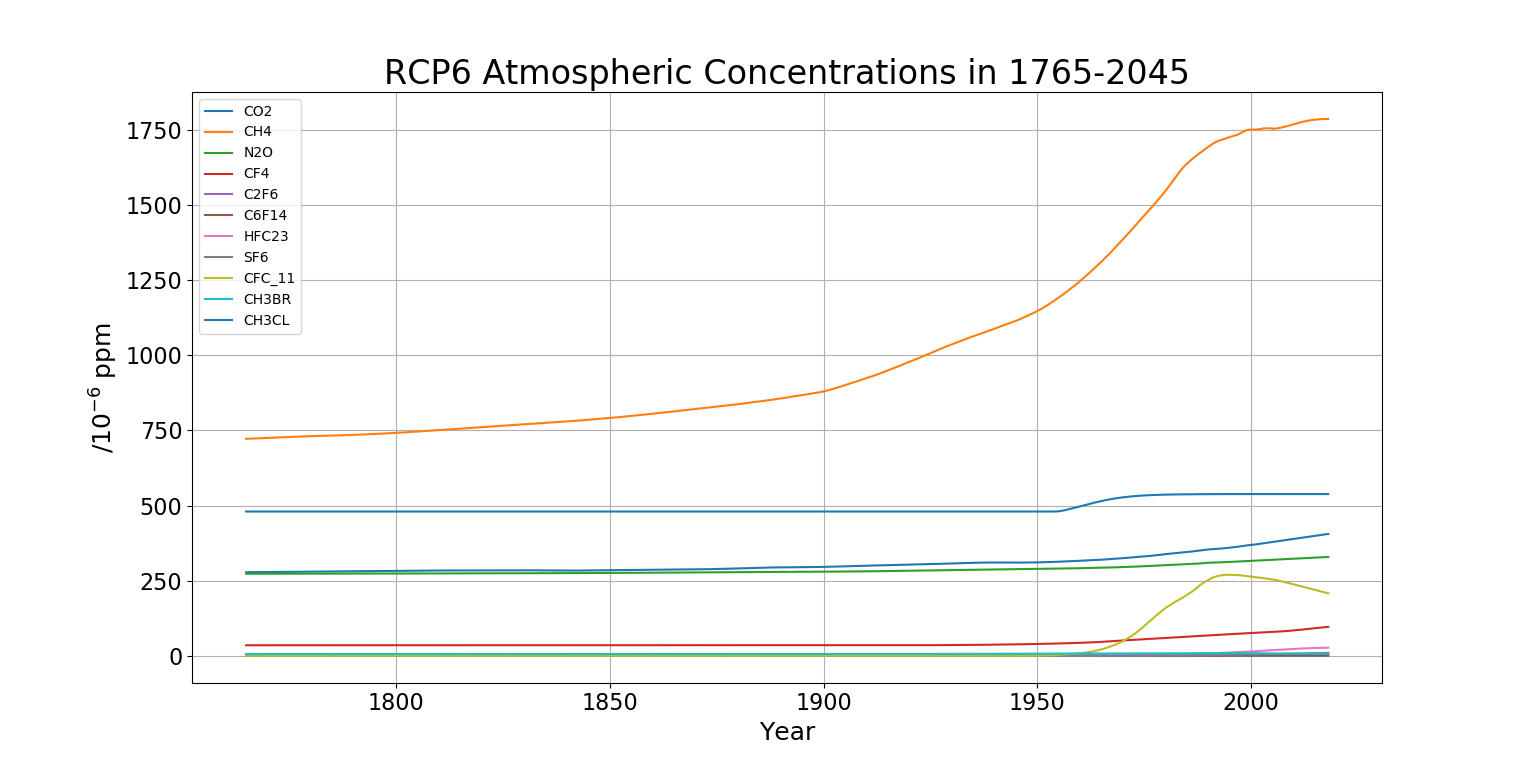
\includegraphics[width=\textwidth]{rcp6_1765_2045.png}
\caption{1765-2045年RCP6预测趋势}\label{rcp6}
\end{figure}

\begin{figure}[!h]
\centering
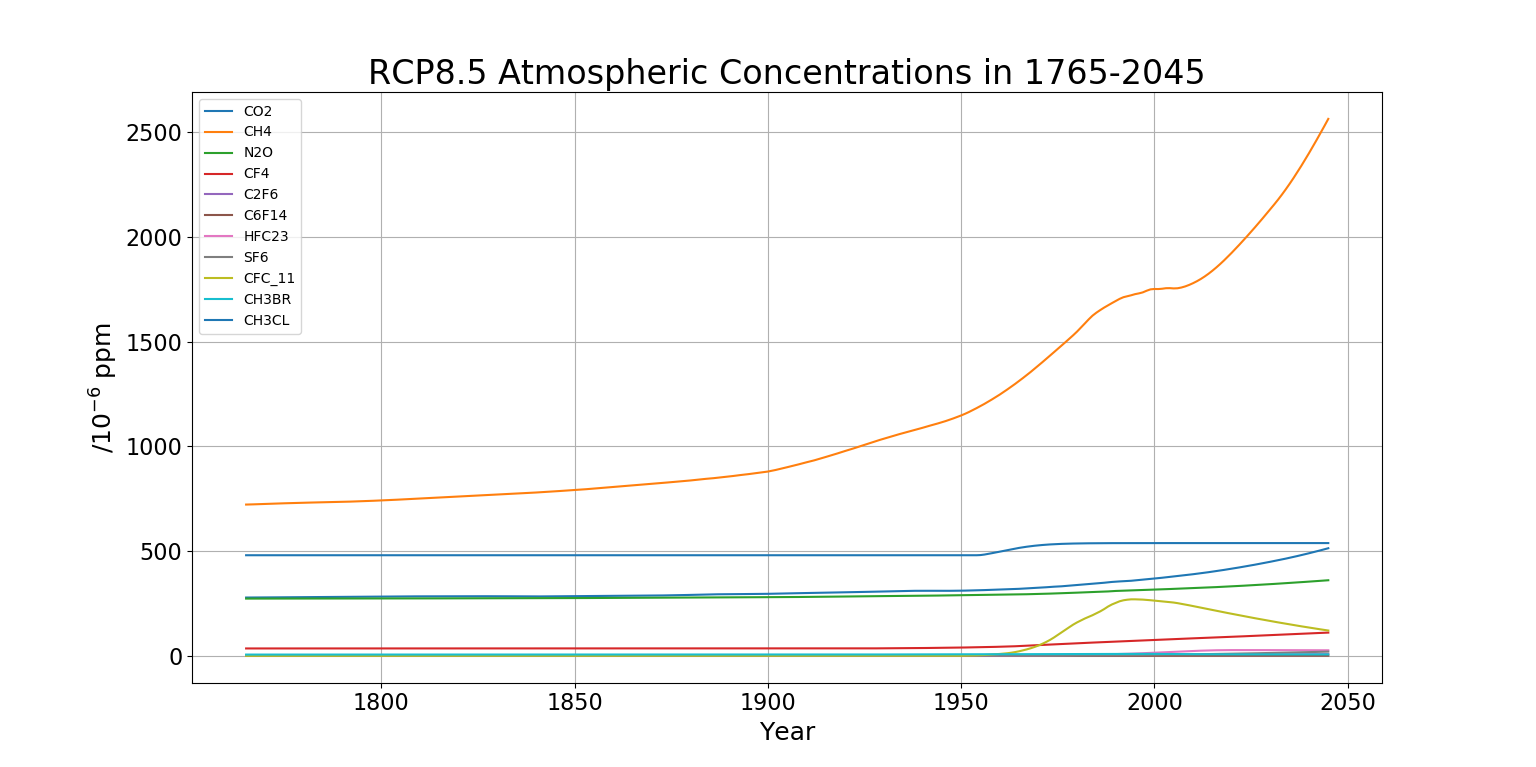
\includegraphics[width=\textwidth]{rcp85_1765_2045.png}
\caption{1765-2045年RCP85预测趋势}\label{rcp85}
\end{figure}

主成分分析方法(principal component analysis,PCA)的主要目的是用较少的变量去解释原来资料中的大部分变异,将RCP中所包含的相关性较高的变量转化成彼此相互独立或不相关的变量,来实现降维。我们以RCP85为样例,首先对其进行标准化,并得到各温室气体之间的相关性矩阵如图\ref{hm}所示。
\begin{figure}[!h]
\centering
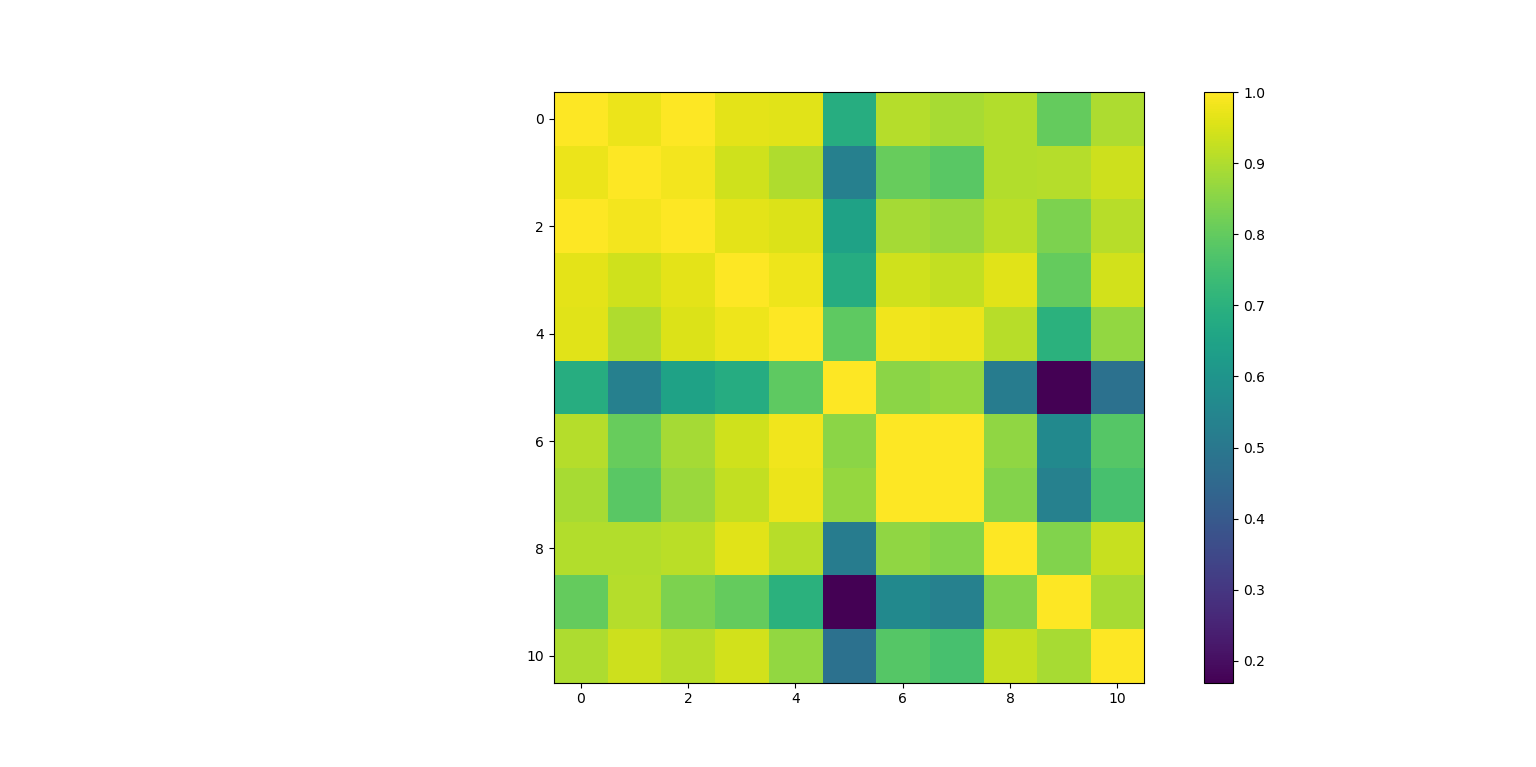
\includegraphics[width=\textwidth]{RCP_heatmap.png}
\caption{各温室气体相关性矩阵}\label{hm}
\end{figure}

对其进行主成分分析,得到各个特征值的方差贡献率如表\ref{RCP_PCA}所示。

\begin{table}[!h]
\centering
\caption{全球RCP PCA分解的前3个特征向量贡献率}\label{RCP_PCA}%添加标题 设置标签
\begin{tabular}{cccccc}
\toprule  %添加表格头部粗线
模态& 特征值& 方差贡献率& 累计方差贡献率& 特征根误差下限& 特征根误差上限\\
\midrule  %添加表格中横线
1& 9.45233733& 0.8593034& 0.8593034& 9.15222532& 9.75244934\\
2& 1.22528405& 0.1113895& 0.9706929& 1.186381243& 1.264186857\\
3& 0.18961885& 0.0172381& 0.9879309& 0.183598441& 0.195639249\\
\bottomrule %添加表格底部粗线
\end{tabular}
\end{table}

其中模态一,所占方差贡献率达到85\%,其对应的时间序列如图\ref{PCA_RCP}所示。我们使用该时间序列表征RCP对于未来25年气候变化的影响。

\begin{figure}[!h]
\centering
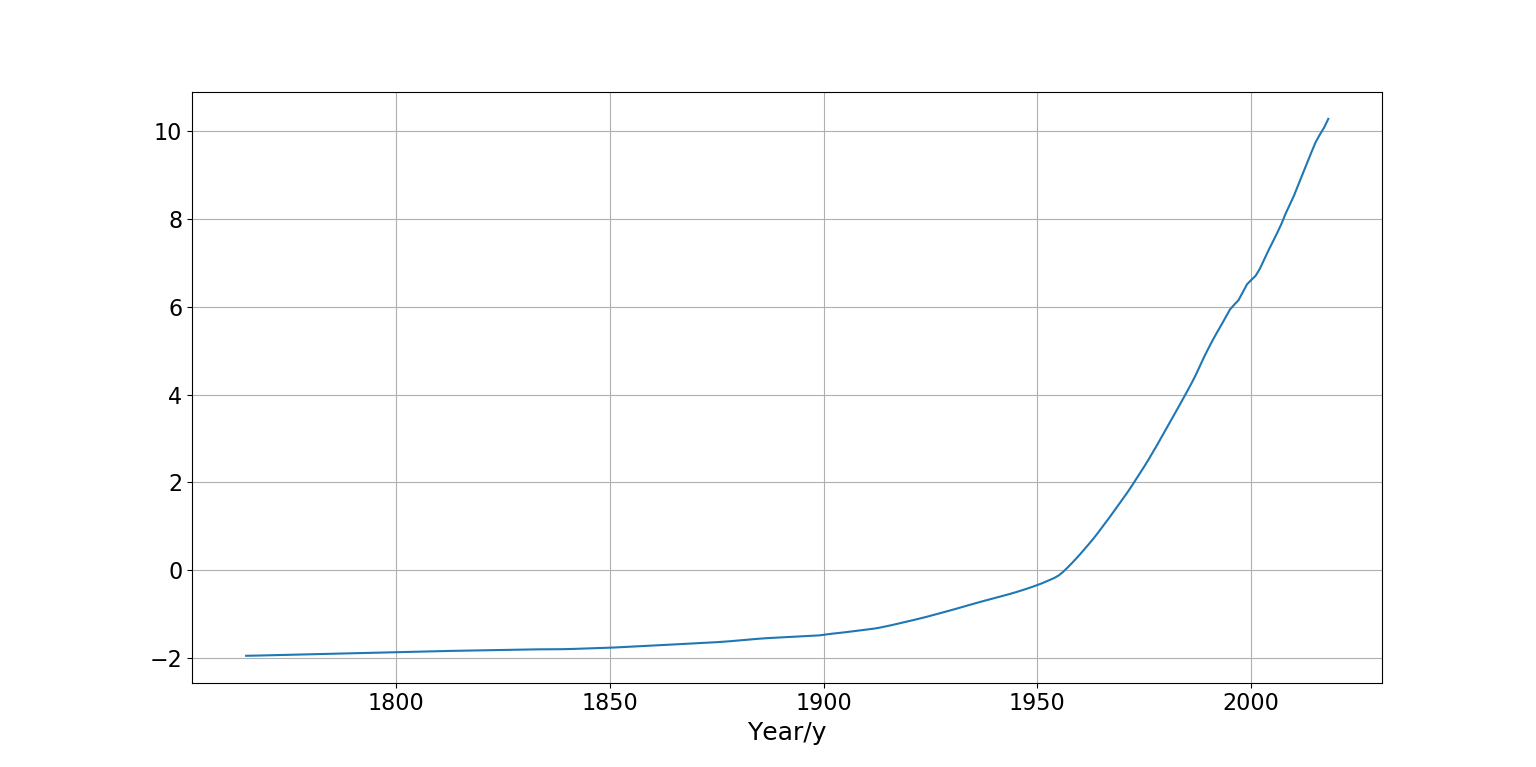
\includegraphics[width=\textwidth]{PCA_RCP.png}
\caption{1765-2045年RCP85预测趋势}\label{PCA_RCP}
\end{figure}

\subsubsection{系统模型的求解}

将海洋表面温度模态与RCP模态带入偏微分方程中,根据RCP的乐观与悲观模型,得到未来25年气温变化趋势如图所示。其中乐观模型表征如果人类社会碳排放量能在最近十年内得到有效控制,RCP浓度将在2050年左右达到峰值。

\begin{figure}[!h]
\centering
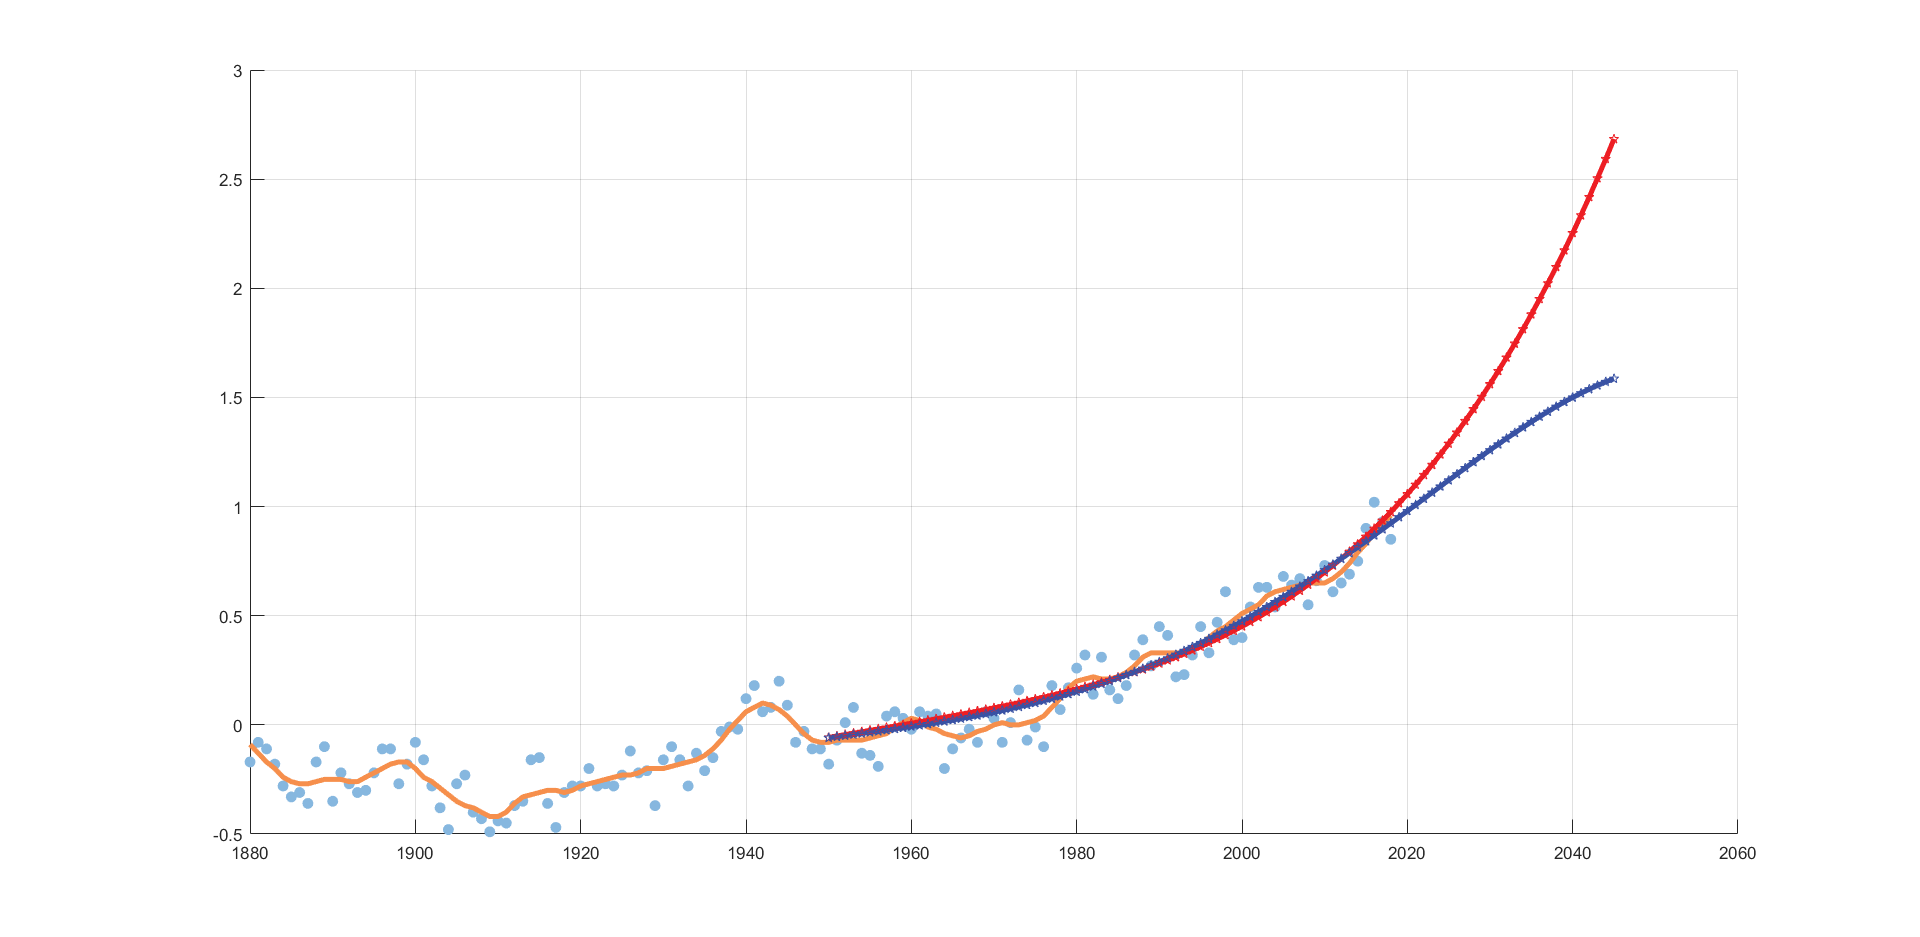
\includegraphics[width=\textwidth]{气温预测.png}
\caption{未来25年气温变化趋势预测曲线}\label{predict}
\end{figure}

\section{问题三分析与建模}

\subsection{问题分析}

问题三要求可分为两部分任务,任务一要求建立模型说明“极寒”天气这种极端天气的出现与气候变化的关系;任务二要求通过模型说明全球变暖与局地极寒现象出现的关系。

针对任务一,我们通过对全球各地历年气温数据进行分析,统计每年各地极寒现象发生次数,从而得出极寒天气与气候变化的关系。

针对任务二,我们运用问题二中全球海洋表面平均温度的EOF模态,解释全球变暖与局地极寒现象出现的关系。

\subsection{问题求解}

运用问题二中全球海洋表面平均温度的EOF模态,结合全球信风以及洋流规律,针对北美地区,我们建立如图\ref{na}所示模型。

\begin{figure}[ht]
\centering
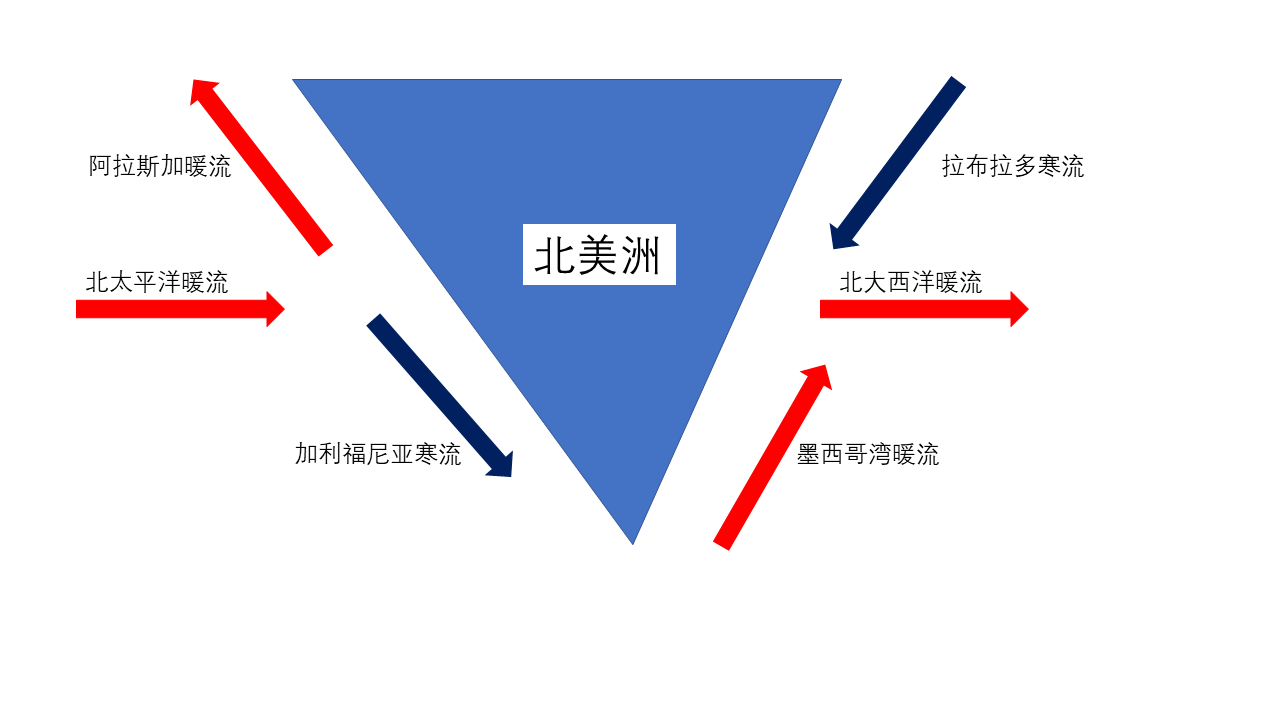
\includegraphics[width=\textwidth]{北美洋流.png}
\caption{北美洋流}\label{na}
\end{figure}

北美洲中高纬度东西海岸地区分别受北太平洋暖流和北大西洋暖流影响,冬季气温较为温和。同时,在极地东风的影响下,北极的冰盖融水向南流动形成拉布拉多寒流。随着温室效应的加剧,全球变暖使得北极冰盖融化加速,大量的冰水混合物从北极受极地东风影响,向西南方向流动,从而造成寒流加剧。冰水混合物在使海洋表面温度保持在0℃左右的同时,遭遇北太平洋暖流与北大西洋暖流,从而不断地融化吸收热量,使得暖流受阻\cite{St2009Climate},最终导致北美中高纬度地区出现局地极寒现象\cite{Nicholls1999Cognitive}。

\section{问题四分析与建模}

\subsection{问题分析}

问题四的要求可分为两部分任务,任务一要求用通俗易懂的文字来解释“今年的冬天特别冷”与“全球变暖”这一气候变化名字之间的关系;任务二要求用一个全新的概念来替代“全球变暖”这一气候变化概念,并且这个概念可以同样反映气候变化的趋势与复杂性。

针对任务一,我们依靠问题三建立的模型推测出的相关结论来初步确定“今年的冬天特别冷”与“全球变暖”之间的关系,再通过第二问的影响要素来进一步推断彼此之间的详细关系。

针对任务二,我们综合考虑问题二、问题三影响气候变化趋势的因素\cite{Palmer2004REPRESENTING}、以及气候变化的影响结果,来创造一个新的名词\cite{St2009Climate},能更好的体现其复杂性\cite{Hastenrath1991Climate}。

\subsection{问题解答}

对于任务一,我们通过问题三建立的模型,发现“极寒天气”这种极端气象的出现与气候变化具有一定的相关性。因此我们基于问题三模型得到的四结论如图\ref{circle}。

\begin{figure}[!h]
\centering
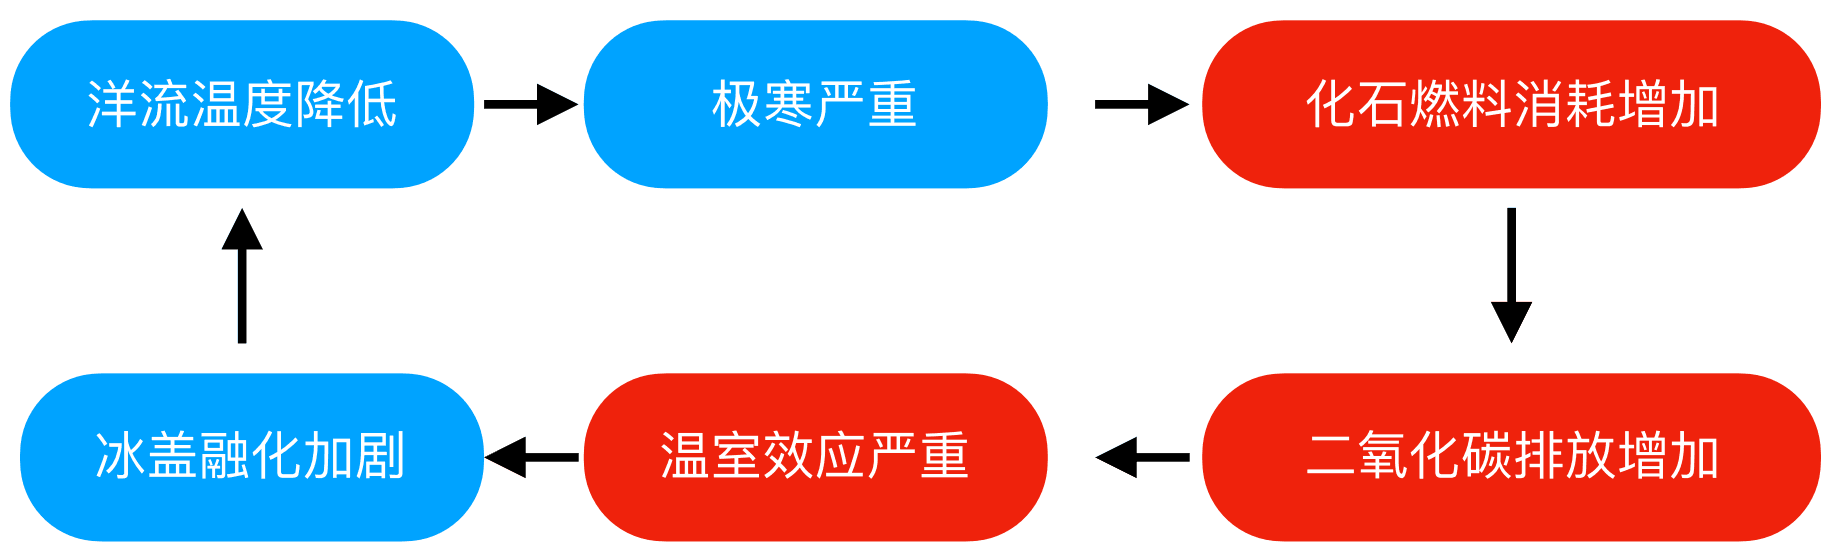
\includegraphics[width=\textwidth]{circle.png}
\caption{“今年的冬天特别冷”与“全球变暖”循环}\label{circle}
\end{figure}

冬天到来时,人们感受到空气变冷,便会增加空调、暖气等发热设备的使用量。这时全球使用化石燃料便会增加,进一步使得碳排放量增加。长时间过高的碳排放量会导致温室效应的加剧,从而致使极地地区冰盖融化加速。冰盖融化变为的冰水混合物流向附近海域。受极低东风影响,冰盖融化的冰水混合物随着洋流运动流向非极地地区,加剧极地寒流,如北美洲东北海岸的拉布拉多寒流。冰水混合物随洋流向中纬度地区流动的同时也在进一步融化吸热,阻碍北太平洋暖流与北大西洋暖流,使得非极地地区的海洋表面与海洋上空大气温度不断下降,最终造成“某年的冬天特别冷”这样的现象。“某年冬天特别冷”又会使人们使用更多的化石燃料取暖,进而形成一个循环\cite{Hastenrath1991Climate}。

如上的这段文字即清晰地解释了“今年的冬天特别冷”与“全球变暖”这一气候变化名字之间的关系。通过这段解释可以看出如果不在该循环任何一个环节加以控制,将会造成非常“不堪设想”的结局。

针对任务二,因为旧概念“全球变暖”会导致全球降水量重新分配、冰川和冻土消融、海平面上升等威胁人类生存的因素,也就是说造成的气候影响是多方面、多维度的,而不仅仅是“变暖”这一层含义,通过问题一到问题三的数据结果也可以印证“全球变暖”不仅仅只代表气温升高这一单一气候变化。但是只有进行相应数据分析与统计的人才能理解到这层含义,所以对于新概念的设定,需要让普通民众也能直接理解他会造成更多不稳定的、极端的气候现象,因此我们定义新概念“全球气候愈发极端”来替代原有“全球变暖”这一概念。此后,不论气温逐年升高、冬季愈发寒冷、台风愈加频繁、冻土不断消融亦或海平面持续上升等,这一系列曾经不出现的自然现象的\cite{Palmer2004REPRESENTING},都可用“全球气候愈发极端”来让民众更好的理解与使用\cite{Hastenrath1995Recent}。


%参考文献   手工录入
%\begin{thebibliography}{9}%宽度9
% \bibitem{bib:one} ....
% \bibitem{bib:two} ....
%\end{thebibliography}

%采用bibtex方案









\bibliographystyle{gmcm}
\bibliography{test}


\newpage
%附录
\appendix
%\setcounter{page}{1} %如果需要可以自行重置页码。
\section{源程序}
\begin{lstlisting}[language=Matlab]%设置不同语言即可。

function [ out ] = slideWindowAve( in, window, stride )
%slideWindowAve
%   in
%   window
%   stride
%   out
len = length(in);
out_len = floor((len - window + 1) / stride);
out = [];
for i = 1 : out_len
    left = i + (i - 1) * (stride - 1);
    right = left + window - 1;
    out(i) = sum(in(left : right)) / window;
end
out = out';
end

function [] = statics_prov(data, provs)
worldmap('canada');
load coast
geoshow(lat, long);
geoshow(provs, 'FaceColor', [1.0 1.0 1.0]);
sorted_data = sort(data);
len = length(data);
p = floor(len / 4);
for i = 1:len
    if data(i) >= sorted_data(len - p + 1)
        color = [249/255 166/255 43/255];
    elseif data(i) >= sorted_data(len - 3 * p)
        color = [77/255 144/255 203/255];
    else
        color = [17/255 59/255 101/255];
    end
    geoshow(provs(i), 'FaceColor', color)
end
end

%%
% 预处理
[nx ny nt] = size(sst);
pre_sst = sst;
% pre_sst(find(isnan(pre_sst)))=0;
pre_sst = reshape(pre_sst, [nx * ny nt]);
%%
% 距平
for i = 1:(nx * ny)
    if ~isnan(pre_sst(i, 1))
        mean_sst = mean(pre_sst(i, :));
        std_sst = std(pre_sst(i, :));
        pre_sst(i, :) = (pre_sst(i, :) - mean_sst) / std_sst;
    else
        pre_sst(i, :) = 0;
    end
end
%%
C = pre_sst * pre_sst' / (nt);
%%
C(find(isnan(C)))=0;
%%
[V lamda] = eig(C);

[nx ny nt] = size(sst);
for i = 1:nx
    for j = 1:ny
        data = sst(i, j, :);
        data = reshape(data, [1, nt]);
        data_1900 = data(600: nt);
        data_1900_1950 = data(600:1200);
        data_1950 = data(1200: nt);
        if ~isnan(data(1))
            sst_std(i, j) = std(data);
            sst_std_1900(i, j) = std(data(600: nt));
            sst_std_1950(i, j) = std(data(1200: nt));
            sst_std_1900_1950(i, j) = std(data_1900_1950);
        else
            sst_std(i, j) = NaN;
            sst_std_1900(i, j) = NaN;
            sst_std_1950(i, j) = NaN;
            sst_std_1900_1950(i, j) = NaN;
        end
    end
end

figure;
hold on;
plot((1:1985), sst_mean, 'o', 'color', [177/255 211/255 238/255],'MarkerFaceColor',[177/255 211/255 238/255]);
plot((1:12:(12*164)), sst_slide_ave, 'color', [54/255 79/255 161/255], 'LineWidth', 3);
sst_slide_ave_5 = slideWindowAve(sst_mean, 12*5, 12);
plot((1:(12):(12*160)), sst_slide_ave_5, 'color', [240/255 31/255 37/255], 'LineWidth', 3);
title('1850-2015年海洋表面平均温度(SST)变化趋势', 'FontSize', 24);
xlabel('/月', 'FontSize', 16);
ylabel('SST/℃', 'FontSize', 16);
legend('月海洋表面平均温度', '年海洋表面平均温度', '年海洋表面滑动平均温度');

figure;
hold on;
plot(t, tm, 'bo');
plot(t(length(t)-length(tma5)+1:length(t)), tma5, 'r-', 'LineWidth', 3);
plot(t(length(t)-length(tma7)+1:length(t)), tma7, 'g-', 'LineWidth', 3);
plot(t(length(t)-length(tma10)+1:length(t)), tma10, 'y-', 'LineWidth', 3);
grid on;
legend('魁北克省12月平均气温', '滑动窗口为5', '滑动窗口为7', '滑动窗口为10');
xlabel('年/year', 'FontSize', 24);
ylabel('T_m /℃ ', 'FontSize', 24);
title('魁北克省12月平均气温滑动滤波效果', 'FontSize', 24);

figure
axesm('eqdcylin','maplatlimit',[-80 80],'maplonlimit',[0 360]);  % Create a cylindrical equidistant map
pcolorm(Nlt,Nlg,sst_std)           % pseudocolor plot "stretched" to the grid
load coast                                 % add continental outlines
plotm(lat,long)
colorbar

%Plot the SST data without using the MATLAB Mapping Toolbox

figure
pcolor(Nlg,Nlt,sst_std);shading interp;
load coast;hold on;plot(long,lat);plot(long+360,lat);hold off
colorbar

figure
axesm('eqdcylin','maplatlimit',[-80 80],'maplonlimit',[0 360]);  % Create a cylindrical equidistant map
pcolorm(Nlt,Nlg,sst_std_1900_1950)           % pseudocolor plot "stretched" to the grid
load coast                                 % add continental outlines
plotm(lat,long)
colorbar

%Plot the SST data without using the MATLAB Mapping Toolbox

figure
pcolor(Nlg,Nlt,sst_std_1900_1950);shading interp;
load coast;hold on;plot(long,lat);plot(long+360,lat);hold off
colorbar

figure
axesm('eqdcylin','maplatlimit',[-80 80],'maplonlimit',[0 360]);  % Create a cylindrical equidistant map
pcolorm(Nlt,Nlg,sst_std_1950)           % pseudocolor plot "stretched" to the grid
load coast                                 % add continental outlines
plotm(lat,long)
colorbar

%Plot the SST data without using the MATLAB Mapping Toolbox

figure
pcolor(Nlg,Nlt,sst_std_1950);shading interp;
load coast;hold on;plot(long,lat);plot(long+360,lat);hold off
colorbar

figure
axesm('eqdcylin','maplatlimit',[-80 80],'maplonlimit',[0 360]);  % Create a cylindrical equidistant map
pcolorm(Nlt,Nlg,model);           % pseudocolor plot "stretched" to the grid
load coast                                 % add continental outlines
plotm(lat,long);
colorbar

\end{lstlisting}

\begin{lstlisting}[language=Python]%设置不同语言即可。

import os
import json

root_path = 'C://Users/hasee007/Desktop/GMCM/'                      # 根目录
data_root = os.path.join(root_path, 'database_canada_tempr_org')    # 数据根目录
result_path = os.path.join(root_path, 'result')                     # 结果目录
json_name = os.path.join(result_path, 'result.json')                # csv结果文件

data_name = ['Tm', 'Tx', 'Tn']
prov_list = ['NS', 'ON', 'QC', 'BC', 'MB', 'NB',
             'NL', 'PE', 'AB', 'SK', 'NT', 'YT', 'NU', 'XX']
month_list = [3, 6, 9, 12]
rcp_list = ['CO2', 'CH4', 'N2O', 'CF4', 'C2F6', 'C6F14', 'HFC23', 'SF6', 'CFC_11', 'CH3BR', 'CH3CL']
data_color = {'Tm': '#CBDEFA', 'Tx': '#FBE5D5', 'Tn': '#CCCCFF',
              'Tm_a': '#2B579A', 'Tx_a': 'orange', 'Tn_a': 'purple'}
is_debug = False


def get_prov_list(data):
    prov_list = []
    for _, value in data.items():
        # print('Key: {}, Value: {}'.format(key, value))
        for prov, _ in value.items():
            if prov not in prov_list:
                prov_list.append(prov)
    print(prov_list)
    return prov_list


import pandas as pd
import numpy as np
from tqdm import tqdm
import os
import json

import config

root_path = config.root_path
is_debug = config.is_debug
data_name = config.data_name

result_path = config.result_path
json_name = os.path.join(result_path, 'result.json')

prov_list = config.prov_list

# main
# data: {'year_month': {'prov': prov_data}}
with open(json_name, 'r') as jobj:
    data = json.load(jobj)

prov_dict = {}
for prov in prov_list:
    dic = {'Year':[], 'Month':[], 'Tm':[], 'Tx':[], 'Tn':[]}
    prov_dict.update({prov: dic})

for key, value in data.items():
    [year, month] = key.split('_')
    for prov, t in value.items():
        prov_dict[prov]['Year'].append(int(year))
        prov_dict[prov]['Month'].append(int(month))
        prov_dict[prov]['Tm'].append(t['Tm'])
        prov_dict[prov]['Tx'].append(t['Tx'])
        prov_dict[prov]['Tn'].append(t['Tn'])

for prov in prov_list:
    prov_path = os.path.join(result_path, '{}.csv'.format(prov))
    df = pd.DataFrame(prov_dict[prov])
    df.sort_values(['Year', 'Month'])
    df.to_csv(prov_path, header=True, index=False)


import pandas as pd
import numpy as np
from tqdm import tqdm
import os
import json

import config

data_root = config.data_root
root_path = config.root_path
is_debug = config.is_debug


def split_filename(filename):
    return filename.split('-')[-1].split('.')[0].split(',')


def get_prov_data(data):
    provs = np.unique(data['Prov'])
    result = {}
    for prov in provs:
        prov_data = data[(data['Prov'] == prov)]
        if is_debug:
            print('{}: \n {}'.format(prov, prov_data))
        prov_result = {}
        for dataName in config.data_name:
            ave = get_ave(prov_data, dataName)
            if is_debug:
                print('{}: {}'.format(dataName, ave))
            prov_result.update({dataName: ave})
        result.update({prov: prov_result})
    return result


def get_ave(data, dataName):
    sum = 0
    cnt = 0
    for index in range(len(data)):
        row_data = data.iloc[index][dataName]
        if not np.isnan(row_data):
            sum += row_data
            cnt += 1
    return sum / cnt if not cnt == 0 else np.nan


# main
result_path = config.result_path
if not os.path.exists(result_path):
    os.mkdir(result_path)

json_name = os.path.join(result_path, 'result.json')

filenames = []
for root, dirs, files in os.walk(data_root):
    for name in files:
        filenames.append(os.path.join(root, name))

all_result = {}
for filename in tqdm(filenames, desc='Read CSV'):
    [month, year] = split_filename(filename)
    print('Solving {} {}'.format(year, month))
    data = pd.read_csv(filename, skiprows=30)
    result = get_prov_data(data)
    if is_debug:
        print('Result for {}-{}:{}'.format(year, month, result))
        break
    json_split_name = os.path.join(
        result_path, '{}_{}.json'.format(year, month))
    with open(json_split_name, 'w') as jobj:
        json.dump(result, jobj)
    all_result.update({'{}_{}'.format(year, month): result})

with open(json_name, 'w') as jobj:
    json.dump(all_result, jobj)

from matplotlib import pyplot as plt

import pandas as pd
import numpy as np
from tqdm import tqdm
import os
import json

import config

root_path = config.root_path
data_root = os.path.join(root_path, 'database_RCP_org')
rcp_list = config.rcp_list
is_debug = True

csv_name = 'RCP85_MIDYEAR_CONCENTRATIONS.csv'
csv_path = os.path.join(data_root, csv_name)

raw_data = pd.read_csv(csv_path, skiprows=37)
year_column = raw_data.columns[0]
data = raw_data[raw_data[year_column] <= 2018]
year = np.array(data[year_column])

plt.figure()
for rcp_kind in rcp_list:
    rcp_data = np.array(data[rcp_kind])
    plt.plot(year, rcp_data, label=rcp_kind)

plt.legend()
plt.grid()
plt.title('RCP8.5 Atmospheric Concentrations in 1765-2045', fontsize=24)
plt.ylabel('/$10^{-6}$ ppm', fontsize=18)
plt.xlabel('Year', fontsize=18)
plt.yticks(fontsize=16)
plt.xticks(fontsize=16)
plt.show()


# coding:utf-8
from matplotlib import pyplot as plt
from tqdm import tqdm

import pandas as pd
import numpy as np
import json
import os

import config

result_path = config.result_path
data_name = config.data_name
data_color = config.data_color
prov_list = config.prov_list
month_list = config.month_list
month_dict = {3: 'Mar.', 6: 'Jun.', 9: 'Sep.', 12: 'Dec.'}

is_debug = False


def slide_window_ave(data, window, stride=1):
    length = len(data)
    out_length = int((length - window + 1) / stride)
    out = []
    for i in range(out_length):
        left = i + (i - 1) * (stride - 1)
        right = left + window
        # print(left, right)
        out.append(np.sum(data[left: right]) / window)
    return out


def show_month_raw_data(data, prov, month):
    year = np.array(data['Year'])
    plt.figure(figsize=(16, 9))
    for name in data_name:
        array = np.array(data[name])
        plt.scatter(year, array, label=name, color=data_color[name])
        ave_array = slide_window_ave(array, window=5)
        # print(len(ave_array), len(year), len(year[-len(ave_array)-1:-1]))
        plt.plot(year[-len(ave_array)-1:-1], ave_array, label='{} 5-year Average'.format(
            name), color=data_color['{}_a'.format(name)], linewidth=3)
    title = 'The Trend of Temperature in {} in {}'.format(
        month_dict[month], prov)
    plt.title(title, fontsize=24)
    plt.legend(loc='best', fontsize=16)
    plt.grid()
    plt.xlabel('Year', fontsize=24)
    plt.ylabel('Temperatue($^\circ C$)', fontsize=24)
    fig_name = '{}_{}.png'.format(prov, month)
    plt.savefig(os.path.join(result_path, fig_name))


def save_statics_data(data, prov, month):
    statics_dict = {}
    for name in data_name:
        array = np.array(data[name])
        mean = np.mean(array[~np.isnan(array)])
        std = np.std(array[~np.isnan(array)])
        statics_dict.update({name: [mean, std]})
    df = pd.DataFrame(statics_dict, index=['mean', 'std'])
    prov_path = os.path.join(result_path, '{}_{}.csv'.format(prov, month))
    df.to_csv(prov_path, header=True, index=True)
    return statics_dict


# main
statics_dict = {}
for prov in tqdm(prov_list, desc='ProvData'):
    prov_dict = {}
    csv_path = os.path.join(result_path, '{}.csv'.format(prov))
    data = pd.read_csv(csv_path)
    # print(data)
    for month in month_list:
        month_data = data[data['Month'] == month]
        # print('month {} \n: {}'.format(month, month_data))
        # show_month_raw_data(month_data, prov, month)
        statics_data = save_statics_data(month_data, prov, month)
        prov_dict.update({month: statics_data})
        if is_debug:
            break
    statics_dict.update({prov: prov_dict})
    if is_debug:
        break

statics_path = os.path.join(result_path, 'statics.json')
with open(statics_path, 'w') as jobj:
    json.dump(statics_dict, jobj)


from matplotlib import pyplot as plt

import pandas as pd
import numpy as np
from tqdm import tqdm
import os
import json

import config

root_path = config.root_path
data_root = os.path.join(root_path, 'database_RCP_org')
rcp_list = config.rcp_list
is_debug = True


def normalization(data):
    _range = np.max(data) - np.min(data)
    return (data - np.min(data)) / _range


def standardization(data):
    mu = np.mean(data, axis=1)
    sigma = np.std(data, axis=1)
    return ((data.T - mu) / sigma).T


def pca(X):
    [_, n] = X.shape
    C = (np.matmul(X, X.T)) / n
    [lamda, v] = np.linalg.eig(C)
    pc = np.matmul(v.T, X)
    return lamda, v, pc, C


csv_name = 'RCP85_MIDYEAR_CONCENTRATIONS.csv'
csv_path = os.path.join(data_root, csv_name)

raw_data = pd.read_csv(csv_path, skiprows=37)
year_column = raw_data.columns[0]
data = raw_data[raw_data[year_column] <= 2018]
year = np.array(data[year_column])

rcp = []
for rcp_kind in rcp_list:
    rcp_data = np.array(data[rcp_kind])
    rcp.append(rcp_data)

rcp = np.array(rcp)

lamda, v, pc, C = pca(standardization(rcp))

plt.figure()
plt.plot(year, pc[0, :])
plt.grid()
plt.xlabel('Year/y', fontsize=18)
plt.yticks(fontsize=16)
plt.xticks(fontsize=16)
plt.show()

plt.imshow(C)
plt.colorbar()
plt.show()

\end{lstlisting}


\end{document}
